\documentclass{article}
\usepackage[utf8]{inputenc}
\usepackage{array}
\usepackage{graphicx}
\usepackage{multirow}
\usepackage{subcaption}
\usepackage{color, colortbl}
\usepackage{float}
\usepackage{hyperref}
\usepackage{setspace}
\usepackage{lipsum}

\usepackage{amsmath}
\usepackage{url,lineno,microtype}

\makeatletter
\g@addto@macro{\UrlBreaks}{\UrlOrds}
\makeatother

\usepackage{fancyhdr}
\pagestyle{fancy}
\fancyhf{}

\newcommand{\SubItem}[1]{
    {\setlength\itemindent{15pt} \item[-] #1}
}

\newcolumntype{P}[1]{>{\centering\arraybackslash}p{#1}}
\newcolumntype{M}[1]{>{\centering\arraybackslash}m{#1}}

\title{wrs_rulebook}
\date{May 2019}

\makeatletter
\newcommand\abtname{About this Rulebook}
\if@titlepage
   \newenvironment{about}{%
       \titlepage
       \null\vfil
       \@beginparpenalty\@lowpenalty
       \begin{center}%
         \bfseries \abtname
         \@endparpenalty\@M
       \end{center}}%
      {\par\vfil\null\endtitlepage}
\else
   \newenvironment{about}{%
       \if@twocolumn
         \section*{\abstractname}%
       \else
         \small
         \begin{center}%
           {\bfseries \abtname\vspace{-.5em}\vspace{\z@}}%
         \end{center}%
         \quotation
       \fi}
       {\if@twocolumn\else\endquotation\fi}
\fi

\newcommand\ackname{Acknowledgements}
\if@titlepage
   \newenvironment{acknowledgements}{%
       \titlepage
       \null\vfil
       \@beginparpenalty\@lowpenalty
       \begin{center}%
         \bfseries \ackname
         \@endparpenalty\@M
       \end{center}}%
      {\par\vfil\null\endtitlepage}
\else
   \newenvironment{acknowledgements}{%
       \if@twocolumn
         \section*{\abstractname}%
       \else
         \small
         \begin{center}%
           {\bfseries \ackname\vspace{-.5em}\vspace{\z@}}%
         \end{center}%
         \quotation
       \fi}
       {\if@twocolumn\else\endquotation\fi}
\fi
\makeatother

\rhead{\includegraphics[width=2cm]{{images/logo_RoboCupAtHome.jpg}}}

\begin{document}
\begin{titlepage}
\begin{figure}[H]
    \begin{tabular}{cc}
      \begin{minipage}[t]{0.5\hsize}
%        \centering
	\raggedright
        \includegraphics[width=2cm]{images/logo_RoboCupFed.jpg}      \end{minipage} &
      \begin{minipage}[t]{0.5\hsize}
%        \centering
	\raggedleft
        \includegraphics[width=2cm]{images/logo_RoboCupAtHome.jpg}
      \end{minipage}
    \end{tabular}
  \end{figure}

	\centering
	%\includegraphics[width=0.15\textwidth]{example-image-1x1}\par\vspace{1cm}
	{\scshape\LARGE RoboCup2021\par}
	\vspace{1cm}
	{\scshape\LARGE @Home\par}
	\vspace{1.5cm}
	{\huge\bfseries Simulation DSLP\par}
	\vspace{2cm}
	{\Large\itshape Rules \& Regulations\par}
	\vfill
	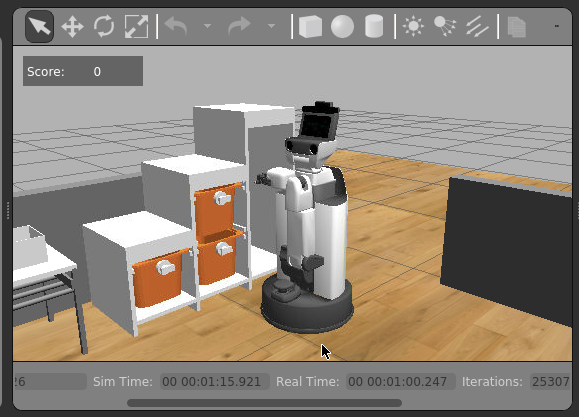
\includegraphics[width=0.80\textwidth]{{images/sim01.png}}
	\vfill
	
% Bottom of the page
%	{\large \today\par}
{\large Version 0.0.0 (January 25, 2021)}
\end{titlepage}

\newpage

\begin{about}

This is the official rulebook of the RoboCup DSPL Simulation 2021 competition. It has been written by the Service Category Technical Committee members.

\end{about}

\begin{acknowledgements}

We would like to thank all the people who contributed to the RoboCup @home Technical Committee members with their feedback and comments. We also like to thank the members of World Robot Summit community.


\end{acknowledgements}

\clearpage
%\doublespacing
\spacing{1.5}
\tableofcontents{}
\singlespacing
\clearpage

\section{Introduction}

\subsection{RoboCup}
RoboCup is an international joint project to promote AI, robotics, and related fields. It is an attempt to foster AI and intelligent robotics research by providing standard problems where a wide range of technologies can be integrated and examined. More information can be found at {\small\url{http://www.robocup.org/}}.

\subsection{@Home}
The RoboCup@Home league aims to develop service and assistive robot technology with high relevance for future personal domestic applications. It is the largest international annual competition for autonomous service robots and is part of the RoboCup initiative. A set of benchmark tests is used to evaluate the robots' abilities and performance in a realistic non-standardized home environment setting. Focus lies on the following domains but is not limited to: Human-Robot-Interaction and Cooperation, Navigation and Mapping in dynamic environments, Computer Vision and Object Recognition under natural light conditions, Object Manipulation, Adaptive Behaviors, Behavior Integration, Ambient Intelligence, Standardization and System Integration. It is colocated with the RoboCup symposium.

\subsection{Domestic Standard Platform League}
The Domestic Standard Platform League(DSPL) has as main goal to assist humans in a domestic environment, paying special attention to elderly people and people suffering of illness or disability.

In consequence, the DSPL focuses on Ambient Intelligence, Computer Vision, Object Manipulation, Safe Indoor Navigation and Mapping, and Task Planning.


\footnotetext[1]{Takashi Yamamoto et. al. \textit{Development of Human Support Robot as the research platform of a domestic mobile manipulator}. ROBOMECH Journal, 2019.}

The robot to be used in the DSPL is Human Support Robot\footnotemark (HSR) by Toyota Motor Corporation shown in  Figure \ref{fig:dspl1} and Figure \ref{fig:dspl2}.

\begin{figure}[!h]
	\centering
	\begin{subfigure}{.45\textwidth}
  		\centering
  		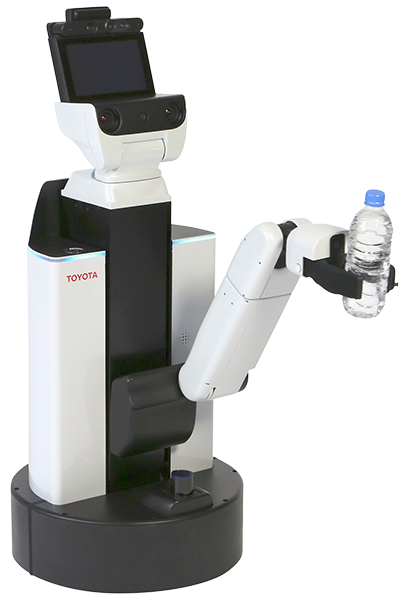
\includegraphics[width=1\textwidth]{{images/real01.png}}
  		\caption{}
  		\label{fig:dspl1}
	\end{subfigure}
	\begin{subfigure}{.30\textwidth}
  		\centering
  		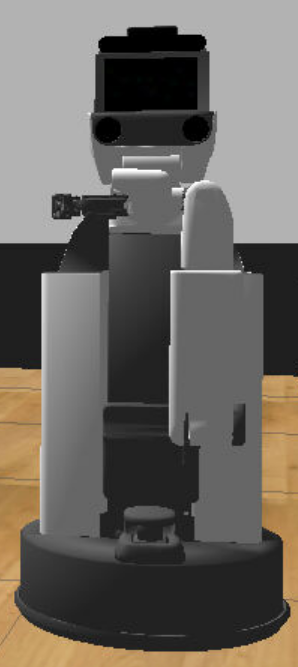
\includegraphics[width=1\textwidth]{{images/real03.png}}
  		\caption{}
  		\label{fig:dspl2}
	\end{subfigure}
	\caption{a) The Toyota Human Support Robot and b) the Simulated model.}
	\label{fig:dspl}
\end{figure}

\clearpage
\section{Simulation DSPL}
\subsection{Concept}

The simulation Domestic Standard Platform League surges from the necessity to standarise and spread the research on Domestic Service Robots where a series of baselines can be tested in a standard benchmark. The simulation league provides a first attempt towards that aim.

\subsection{Competition}

The rules and regulations of the sDSPL are highly based on the World Robot Summit - Partner Robot Challenge (Real Space), as in {\small\url{https://worldrobotsummit.org/}}, and therefore some rules might not be applicable to a simulated environment, especially those limited by real physical and mechanical principles.

\vspace{5mm} %5mm vertical space
\textbf{Simulator}

The TC finally decided to use the OSS HSR simulator. You can find a Docker image of the simulator here:

\vspace{5mm}
{\small\url{https://github.com/hsr-project/hsrb_robocup_dspl_docker}}
{\small\url{https://github.com/devrt/robocup2021-opl}}

\vspace{5mm}
This link\footnotemark explains how to use it in the simulation league.

\footnotetext[2]{{\small\url{http://humansupportrobot.org/}}}

\vspace{5mm}
\textbf{Tests}

The competition is as follows:

\begin{itemize}
    \item Poster Session
    \item Stage I
        \SubItem{Clean Up (5 min)}
        \SubItem{Go and Get It (5 min)}
    \item Stage II
        \SubItem{Clean Up (15 min)}
    \item Final
\end{itemize}

\subsection{Disclaimer}

The Open Source Software of the HSR is provided at it is. The Docker container works under Ubuntu 18.04 and the private Toyota Motor Company libraries are not compatible with the OSS and may cause the system to crash. If you are a regular user of the real robot, please consider this condition when using your code as you might need to adapt your code to the provided libraries.

\clearpage
\section{General Rules}

\subsection{Objectives}
\begin{itemize}
    \item Clean Up: Tidy up objects from the incorrect locations to a predetermined deposit.
    \item Go and Get It: Provide a person within a group with some food from a shelf when requested while avoiding obstacles when navigating.
\end{itemize}

\subsection{Technical Focus}
\begin{itemize}
    \item Semantic mapping, unknown object perception and manipulation, path planning.
    \item HRI, semantic mapping, object manipulation, motion and path planning.
\end{itemize}

\subsection{Vision}

By providing an easy to understand challenge, we aim at identifying and solving front-end problems that might arise when using a service robot in indoors environments, such as safety and stability, autonomous error recovery, task performance and time consumption, natural motion and path planing, etc.

The Key Performance Indicator is based on a 4S philosophy: Speed, Smooth/ Smart, Stable, and Safe.

\subsection{Setup}
\noindent
\textbf{Arena}
\begin{itemize}
    \item The room layout and furniture positions will be as in as in Figure \ref{fig:arena} and the furniture models are presented in Appendix \ref{sec:furniture}.
    \item Each Task is carried out in the following rooms:
        \SubItem{Room 1: Living room (Clean Up), a 3.5x4.0 meters area, with a 1.2m long door in the top left side of the wall working as a main entrance and a 1.2m long free access (i.e. without door) in the bottom of the shared wall connecting to the dining room, as shown in Figure \ref{fig:tidyup}.}
        \SubItem{Room 2: Dining room (Go and Get It), a 2.5x4.0 meters area, as illustrated in Figure \ref{fig:bringdrink}.}
\end{itemize}

\begin{figure}[!h]%[!htbp]
	\centering
	%\begin{center}
	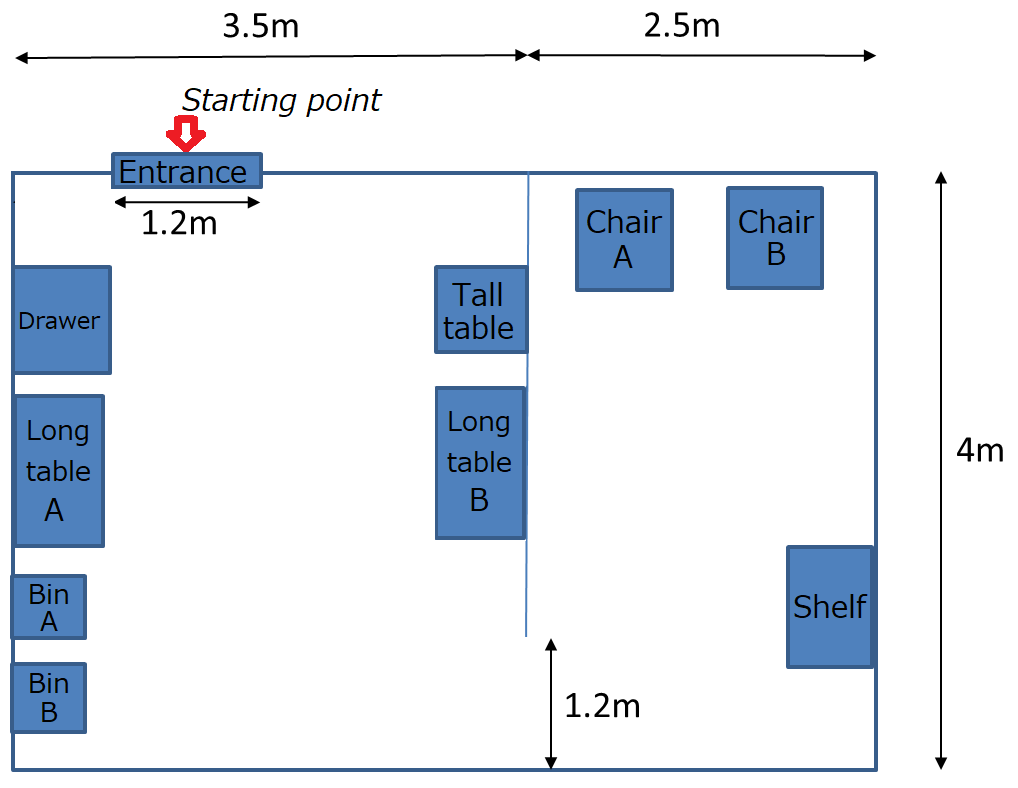
\includegraphics[width=0.80\textwidth]{{images/map.png}}
	\caption{Test arena layout. The red arrow indicates the starting point at the beginning of the competition or after a restart.}
	\label{fig:arena}
	%\end{center}
\end{figure}

\begin{figure}[!h]
	\centering
	\begin{subfigure}{.45\textwidth}
  		\centering
  		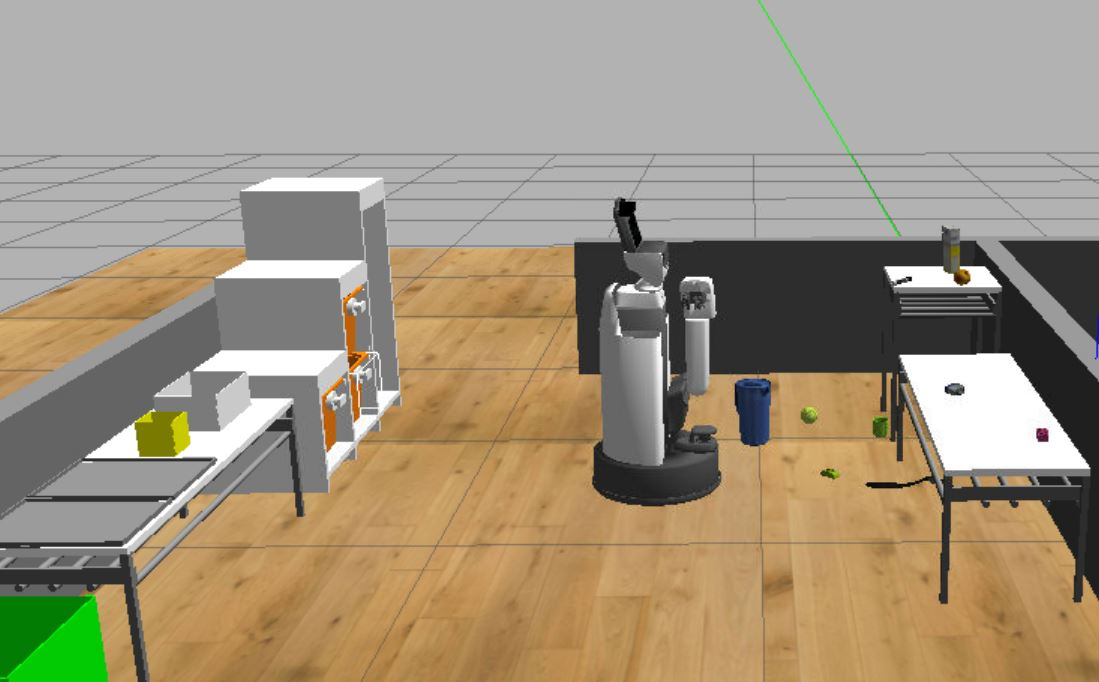
\includegraphics[width=1\textwidth]{{images/tidy_up.jpg}}
  		\caption{}
  		\label{fig:tidyup}
	\end{subfigure}
	\begin{subfigure}{.385\textwidth}
  		\centering
  		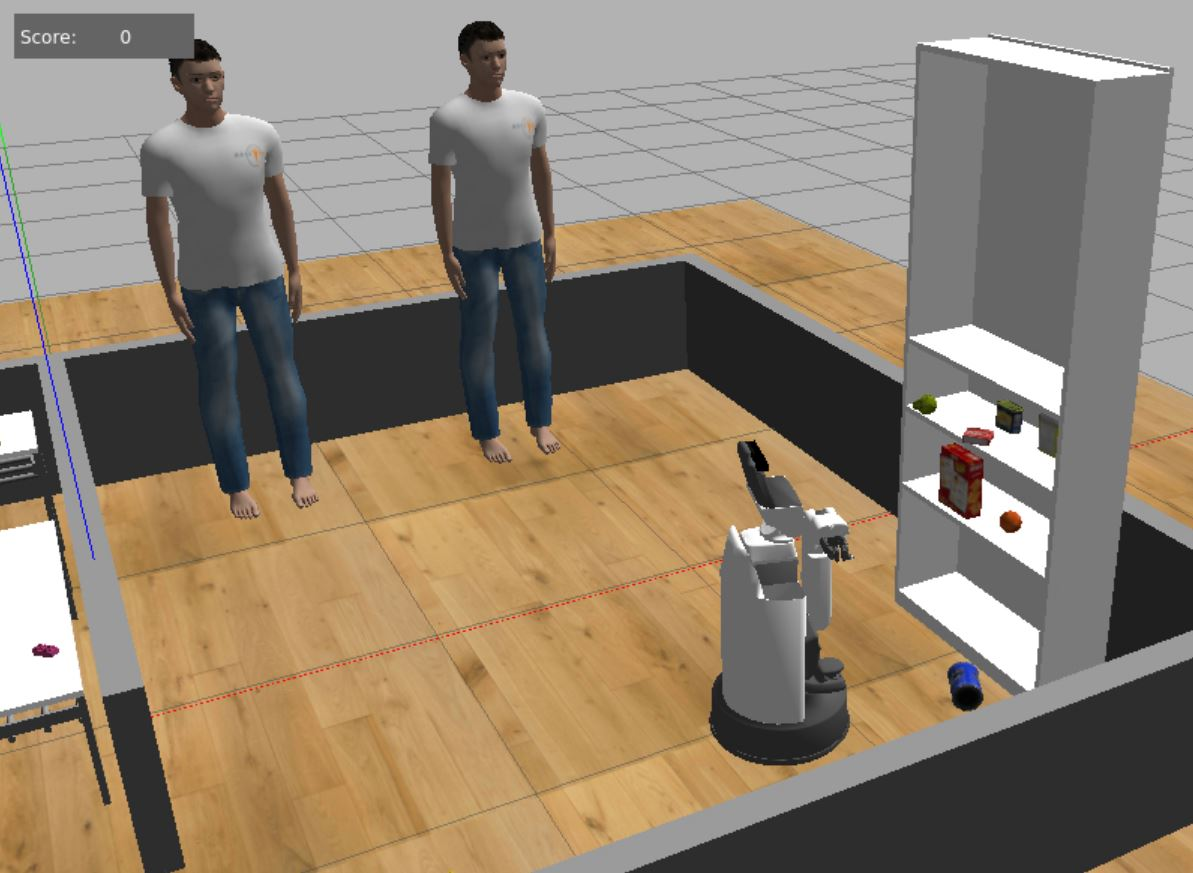
\includegraphics[width=1\textwidth]{{images/bring_drink.jpg}}
  		\caption{}
  		\label{fig:bringdrink}
	\end{subfigure}
	\caption{a) Living room where objects are scattered about. b) Dining room with a shelf and two chairs. For ease of visibility for the audience, \textbf{the wall will have a minimum height of 60 cm}.}
	\label{fig:wrschallenge}
\end{figure}

\noindent
\textbf{Objects}
\begin{itemize}
    \item Known objects - with pre-announced object recognition data and location information --, 25 units in 5 categories\footnotemark (each category has 5 units randomly chosen from the dataset; the selection process is performed per test): 
        \SubItem{Food (e.g. chips can, coffee can, cracker box), kitchen items (e.g. glass, bowl, mug), tools (e.g. clamps, padlock's keys), shape items (e.g. baseball, tennis ball), and task items (e.g. Rubick’s cube, t-shirt, airplane toy)}
    \item Orientation-based items. It is \textbf{important} to notices the existence of this property, where exclusively the following objects have it: 
        \SubItem{small marker: tip faces downwards}
        \SubItem{large marker: tip faces downwards}
        %\SubItem{scissors: tip of blade faces downwards}
        %\SubItem{knife: handle faces upwards}
        \SubItem{fork: handle faces upwards}
        \SubItem{spoon: handle faces upwards}
    \item Unknown objects - without pre-announced object recognition data nor location information. They will be frequently used daily goods and tools as in Young Sang Choi et. al. \footnotemark, and may include deformable objects such as clothing, food, magazines, etc., 5 units (one per category). 
\end{itemize}

\footnotetext[3]{Berk Calli et. al. \textit{Benchmarking in Manipulation Research: The YCB Object and Model Set and Benchmarking Protocols}. IEEE Robotics and Automation Magazine, 2015.}

\footnotetext[4]{Young Sang Choi et. al. (2009), \textit{A list of household objects for robotic retrieval prioritized by people with ALS}. IEEE International Conference on Rehabilitation Robotics, ICORR 2009.}

%\footnotetext[3]{http://www.ycbbenchmarks.com/}

Object's specifications and their corresponding 3D models can be found in http://www.ycbbenchmarks.com/ .

\clearpage
\subsection{Clean Up}

\textbf{Description:} Move the objects spread around a room to their designated locations.

\textbf{Time:} 5 min in Stage I and 15 min in Stage II

\subsubsection{Settings}

\textbf{Environment}
\begin{itemize}
    \item Furniture: stairs-like drawer (Figure \ref{fig:drawer}), long table (x2), tall table, bin (x2).
    \item Storage places: drawer, tray, bin, pen pencil holder (Figure \ref{fig:containers}).
\end{itemize}

\begin{figure}[!h]%[!htbp]
	\centering
	\begin{subfigure}{.365\textwidth}
  		\centering
	    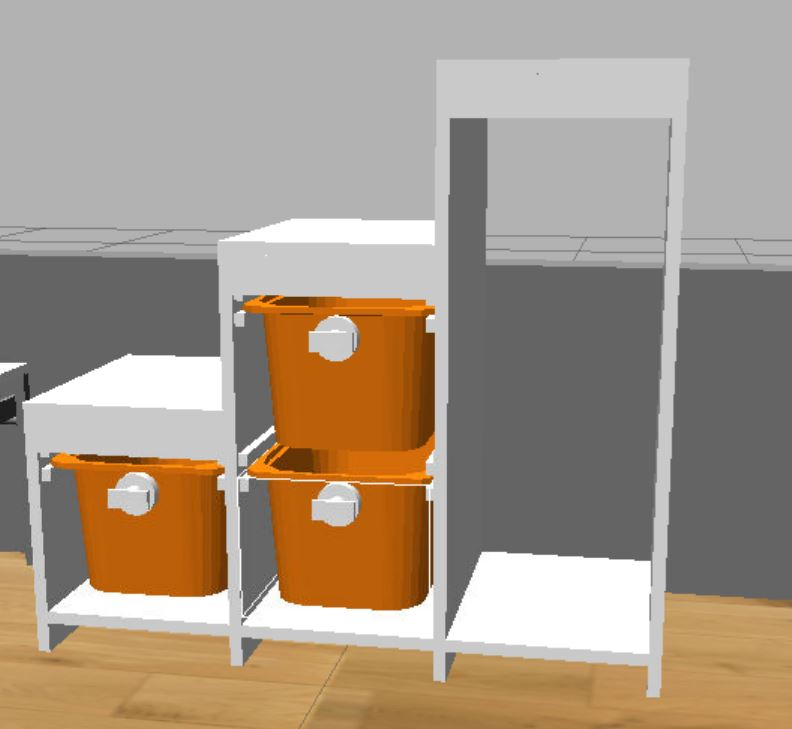
\includegraphics[width=1\textwidth]{{images/drawer.jpg}}
	    \caption{}
  		\label{fig:drawer}
	\end{subfigure}
	\begin{subfigure}{.45\textwidth}
  		\centering
  		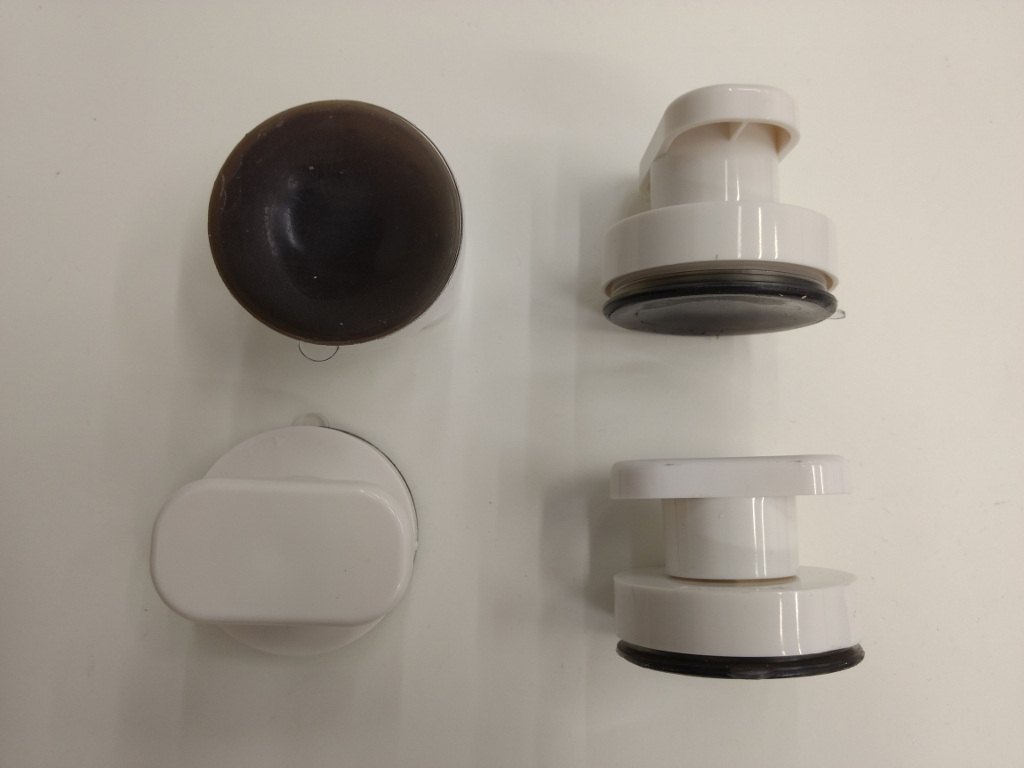
\includegraphics[width=1\textwidth]{{images/handles_b.jpg}}
  		\caption{}
  		\label{fig:handles}
	\end{subfigure}
	\caption{a) Stairs-like drawer. The drawer will be as it is (left drawer) or it might have a handle and/or be opened under team request (middle drawers); when opening a drawer, it should not be unmounted from the shelf. b) Several views of the easy-to-manipulate handles (\url{https://www.amazon.com/Suction-BYBYCD-Handles-Bathroom-Adsorbent/dp/B07GYKJCTR}).}%; as a reference, the circular base has a diameter of 6cm and a height of 2cm while the handle part has a long side of 6cm, short side of 3.5cm and a height of 3cm.}
	\label{fig:fulldrawer}
	%\end{center}
\end{figure}

\begin{figure}[!h]%[!htbp]
	\centering
	%\begin{center}
	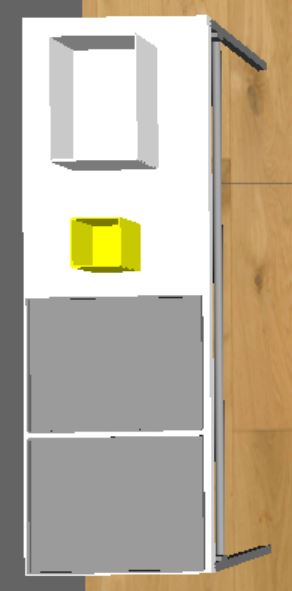
\includegraphics[angle=-90, width=0.80\textwidth]{{images/tray_container.jpg}}
	\caption{Containers may vary in shape and size, but they will be within a predefined area in the deposit area.}
	\label{fig:containers}
	%\end{center}
\end{figure}

\noindent
\textbf{Task Performance}
\begin{itemize}
    \item The name and location of the deposits are fixed, such as tools drawer, food tray, task items bin, kitchen items container, etc.
    \item Known objects are given with pre-announced information on their corresponding deposits. Orientation-based items can be placed in a deposit corresponding to their category (correct category point) or property (correct category and, if correctly placed, orientation points).
    \item The furniture doors will have easy-to-manipulate handles (as in Figure \ref{fig:handles}).
\end{itemize}

\subsubsection{Before the Competition}

\begin{itemize}
    \item Teams are given the time to create/adjust map data in the actual apartment.
    \item Right before the competition, the referee sets the rooms into messy condition (within a specified error tolerance range).
    \item Room 1. Living room (task planning, object recognition and manipulation), for the Clean Up task:
        \SubItem{30 objects (5 categories, 5 known + 1 unknown objects per category) are randomly placed in the room (on the floor and or tables).}
\end{itemize}

\subsubsection{During the Competition}

The robot enters the living room in a messy condition, tidies up the room in 5 minutes (Stage I) or 15 minutes (Stage II). Three runs are allowed per trial. A detailed description of a full run is described below:

\begin{itemize}
    \item Each test starts with the robot at the front entrance (starting point). The start signal is the robot motion.
    \item As the name of the task suggests, the robot should move at least one object to a deposit before being granted any point point (including bonus points). The robot should inform the operator whether the tasks have been completed or the time limit is up.
    \item Clean Up
        \SubItem{Start the competition by moving the robot from the initial position.}
        \SubItem{Perform clean up.}
\end{itemize}

\subsubsection{Scores} \label{sec:scores}

\begin{itemize}
    \item Clean Up
        \SubItem{Grasping an object inside the room and correctly depositing it in a location. It is considered a successful grasping if the robot is able to bring the object to a deposit area; if the robot drops the object in its way to a deposit, it is considered unsuccessful and will be subject to a penalisation (hint: the robot can take a dropped object again); a successful deposit consist on the object being inside the deposit, as in Figure \ref{fig:delivery}. Special consideration is given to clothing and textiles, where they can hang in the deposit's border, but without touching the floor (Figure \ref{fig:cloths}): 10 points x 30 units.}
        \SubItem{Correctly depositing an object according to its category: 10 additional points per object.}
        \SubItem{Correctly depositing an object based on its orientation (e.g. markers' tips facing downwards as in Figure \ref{fig:orientation}): 10 additional points per object.}
        \SubItem{Correctly finishing the task within the time limit (i.e. all objects in the search area have been placed in their corresponding deposit): 50 points.}
    \item The best execution (highest scored run) will be taken as score for that particular trial.
\end{itemize}

\begin{figure}[!h]
\centering
	\begin{subfigure}{.30\textwidth}
  		\centering
  		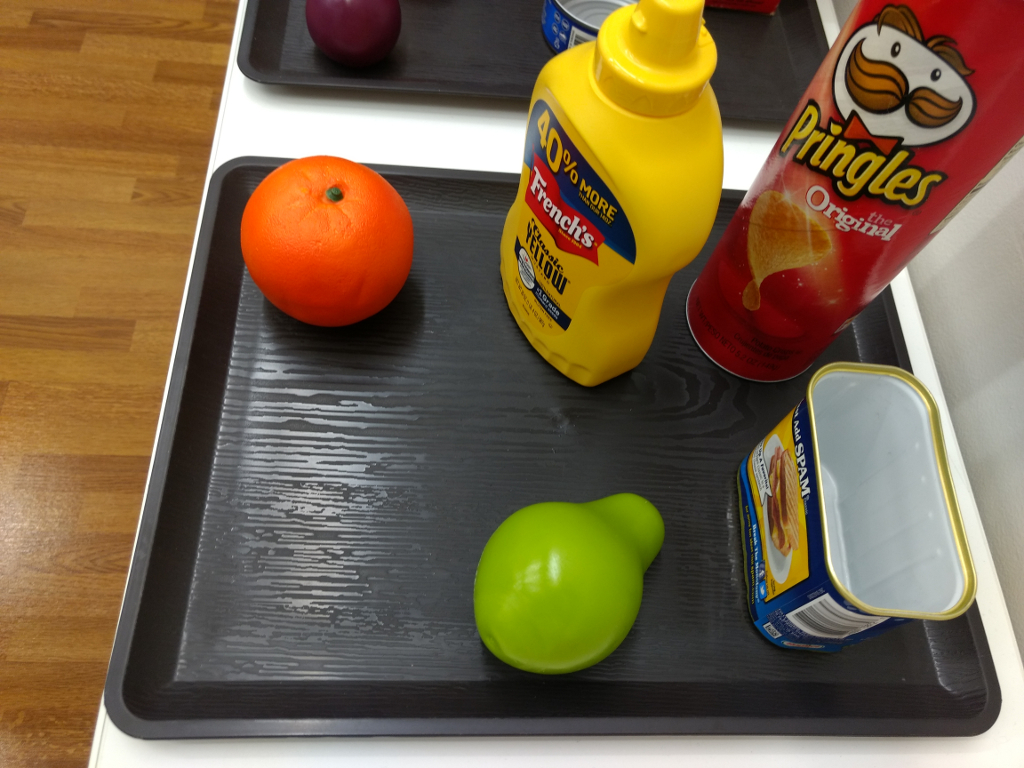
\includegraphics[width=1\textwidth]{{images/tray_setup.jpg}}
  		\caption{}
  		\label{fig:deliverysetup}
	\end{subfigure}
	\begin{subfigure}{.30\textwidth}
  		\centering
  		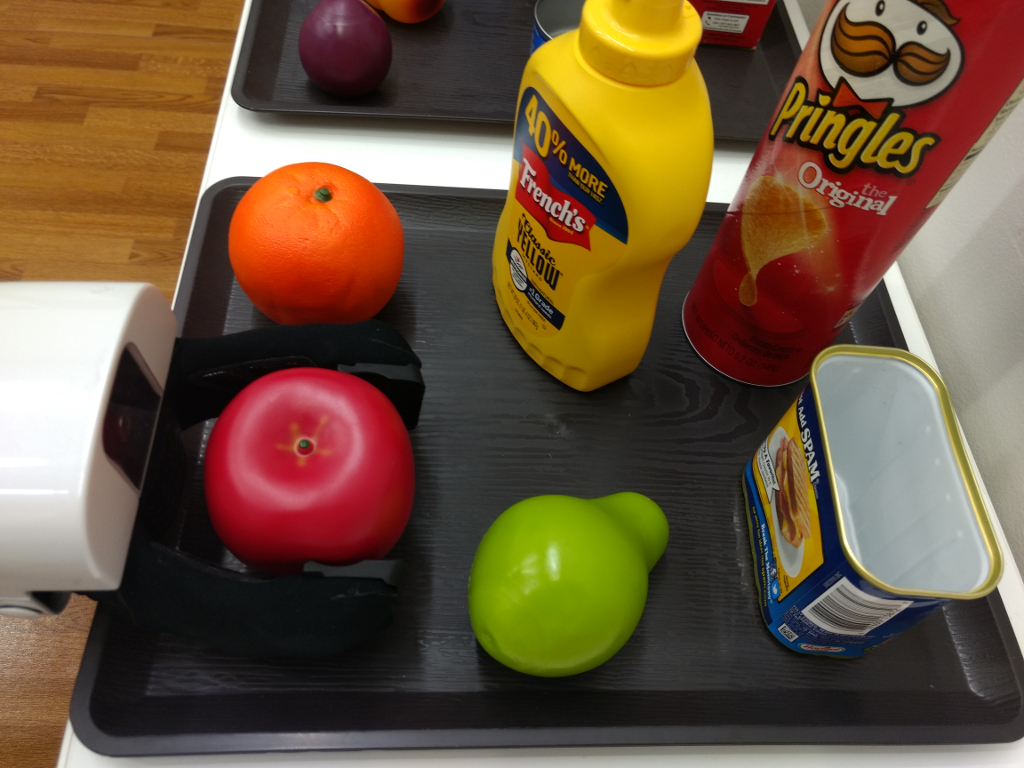
\includegraphics[width=1\textwidth]{{images/tray_correct.jpg}}
  		\caption{}
  		\label{fig:deliverycorrect}
	\end{subfigure}
		\begin{subfigure}{.30\textwidth}
  		\centering
  		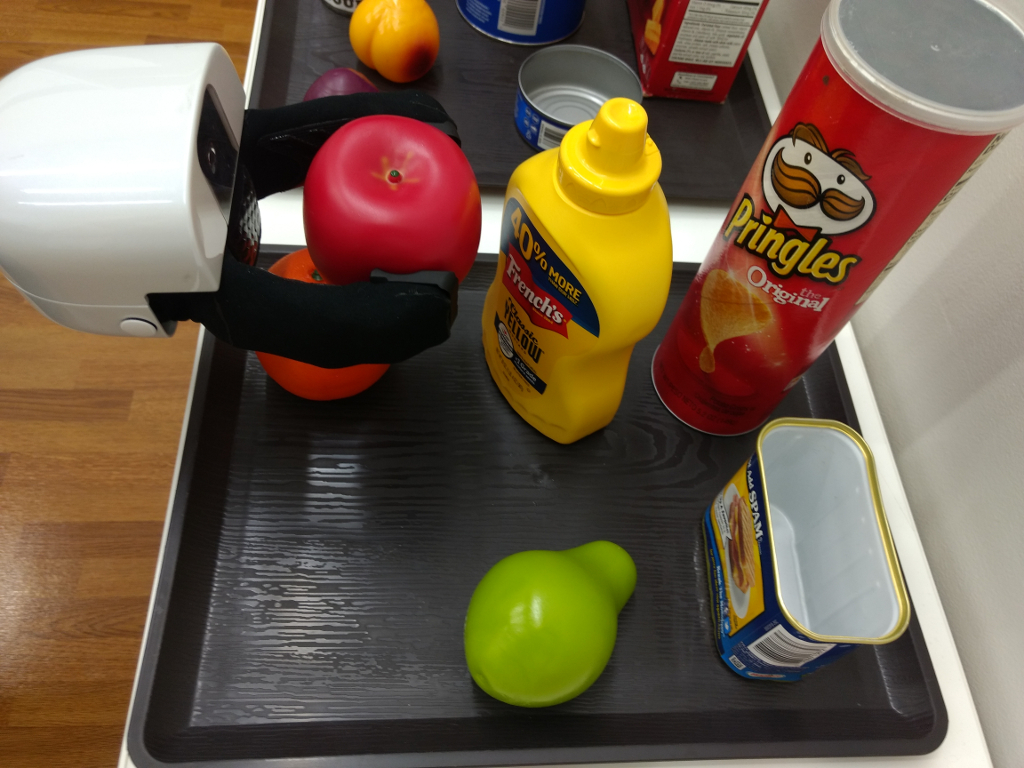
\includegraphics[width=1\textwidth]{{images/tray_wrong.jpg}}
  		\caption{}
  		\label{fig:deliverywrong}
	\end{subfigure}
	\caption{Example of a delivery process in a tray case: a) given a target deposit with objects in it, b) it is considered a correct delivery if the objects is placed softly in a free space, and c) a hit if it is placed in a occupied space. In any case, if, in its final position, a given object touches the table or it doesn't touch the tray (a piling situation where one object is over another), it is considered a failed delivery (zero points for that object).}
	\label{fig:delivery} 
\end{figure}

\begin{figure}[!h]
	\centering
	\begin{subfigure}{.45\textwidth}
  		\centering
  		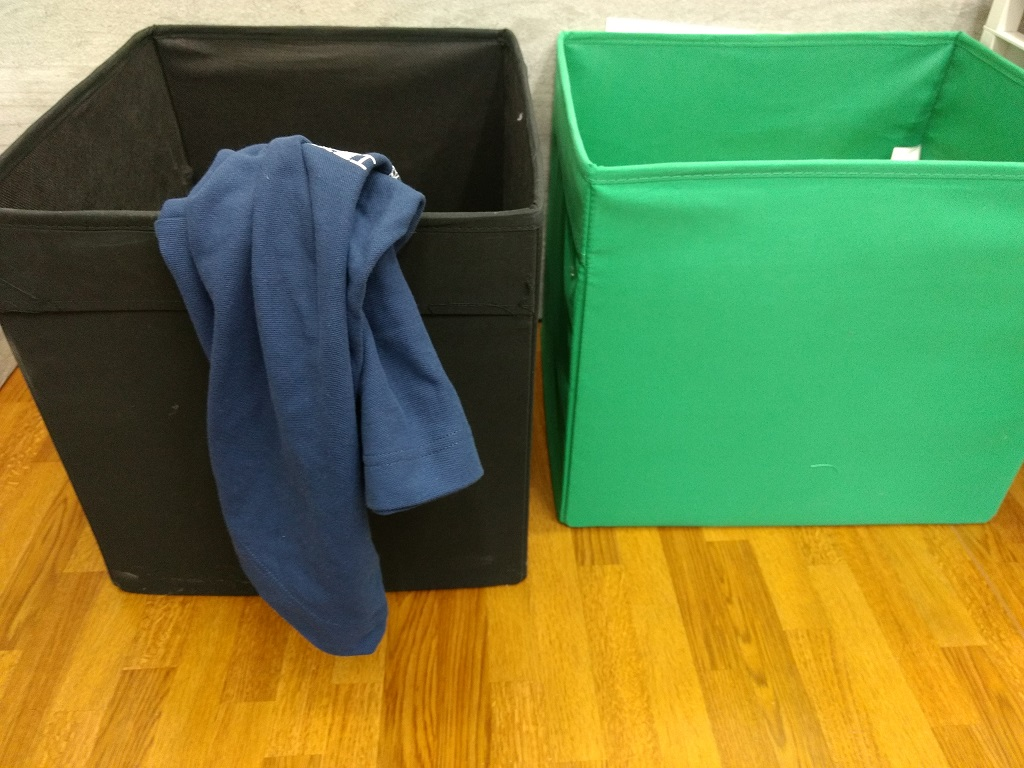
\includegraphics[width=1\textwidth]{{images/cloths_correct.jpg}}
  		\caption{}
  		\label{fig:clothscorrect}
	\end{subfigure}
	\begin{subfigure}{.45\textwidth}
  		\centering
  		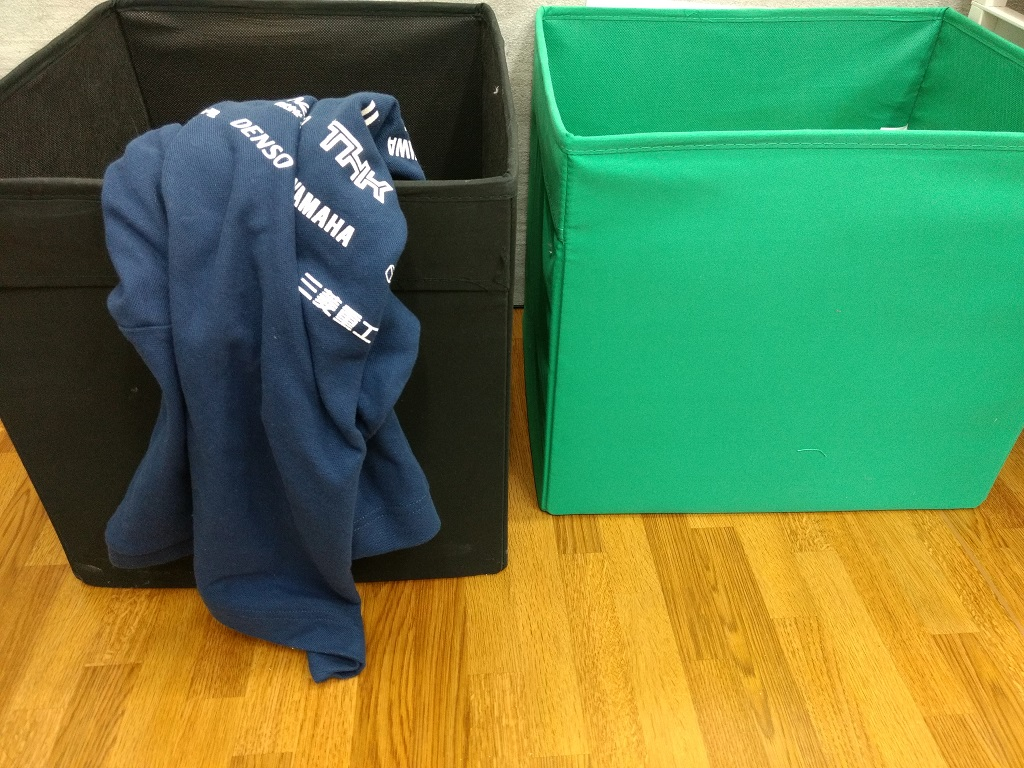
\includegraphics[width=1\textwidth]{{images/cloths_wrong.jpg}}
  		\caption{}
  		\label{fig:clothswrong}
	\end{subfigure}
	\caption{In the case of drawers, containers, and bins, a correct delivery is considered if the objects are inside them in any position. In the special case of clothes, it is consider a) a correct delivery (no contact with the floor) and b) an incorrect delivery.}
	\label{fig:cloths}
\end{figure}

\begin{figure}[!h]%[!htbp]
\centering
	\begin{subfigure}{.30\textwidth}
  		\centering
  		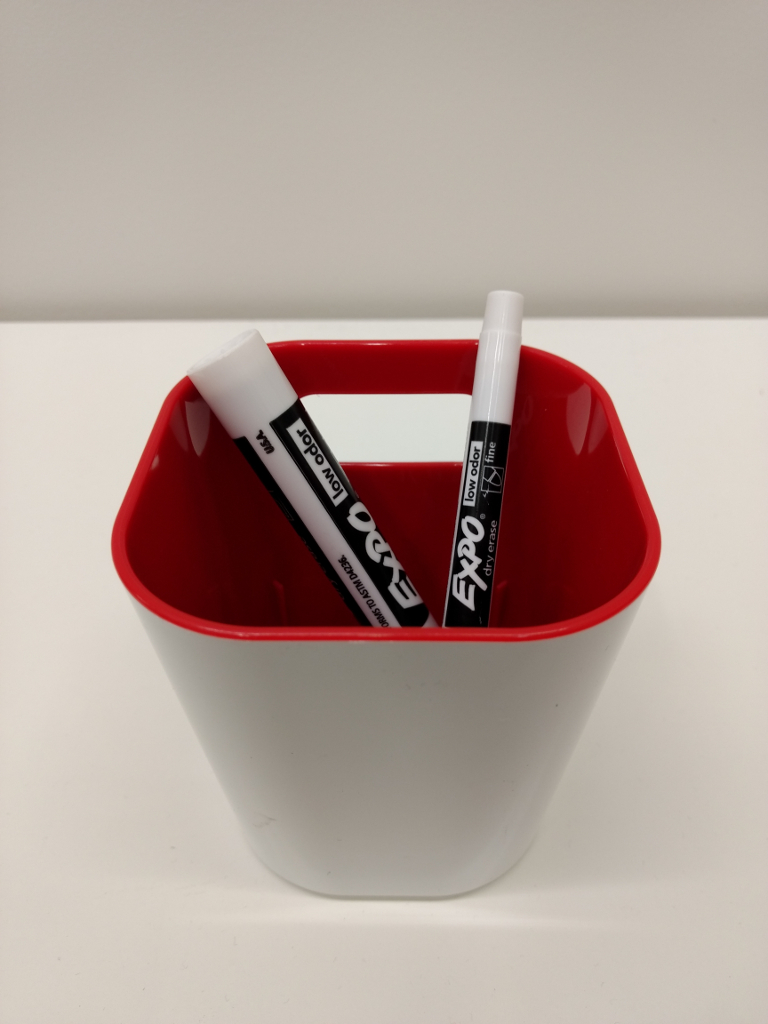
\includegraphics[width=1\textwidth]{{images/orientation_good_1.jpg}}
  		\caption{}
  		\label{fig:orientationgood1}
	\end{subfigure}
	\begin{subfigure}{.30\textwidth}
  		\centering
  		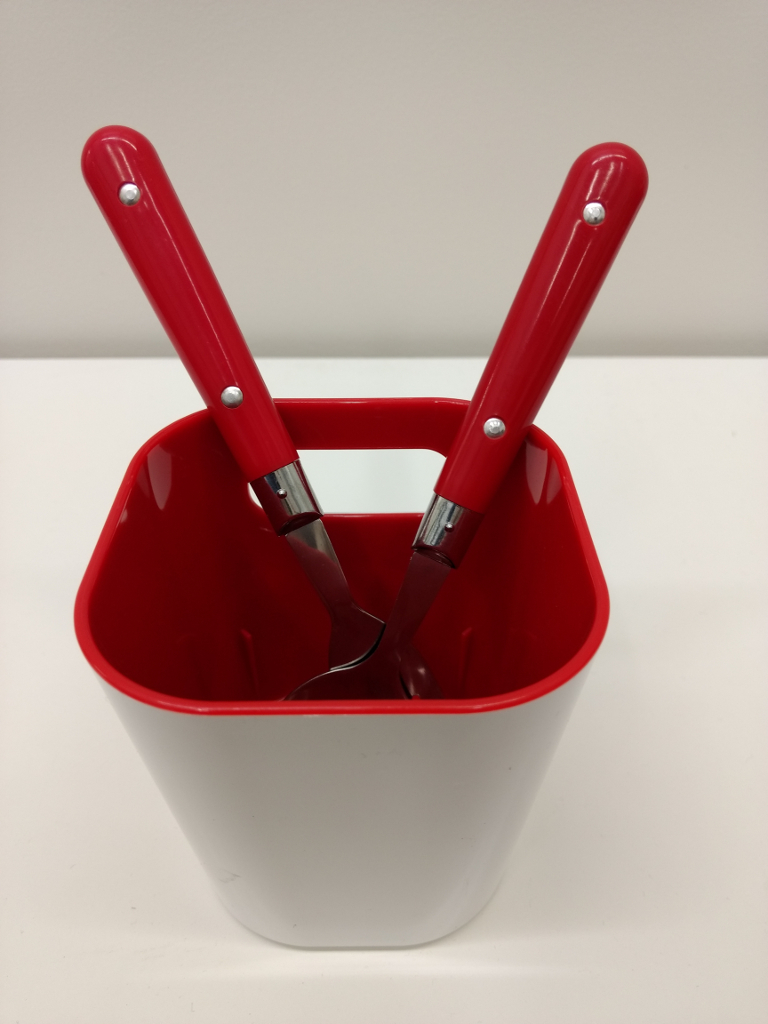
\includegraphics[width=1\textwidth]{{images/orientation_good_2.jpg}}
  		\caption{}
  		\label{fig:orientationgood2}
	\end{subfigure}
		\begin{subfigure}{.30\textwidth}
  		\centering
  		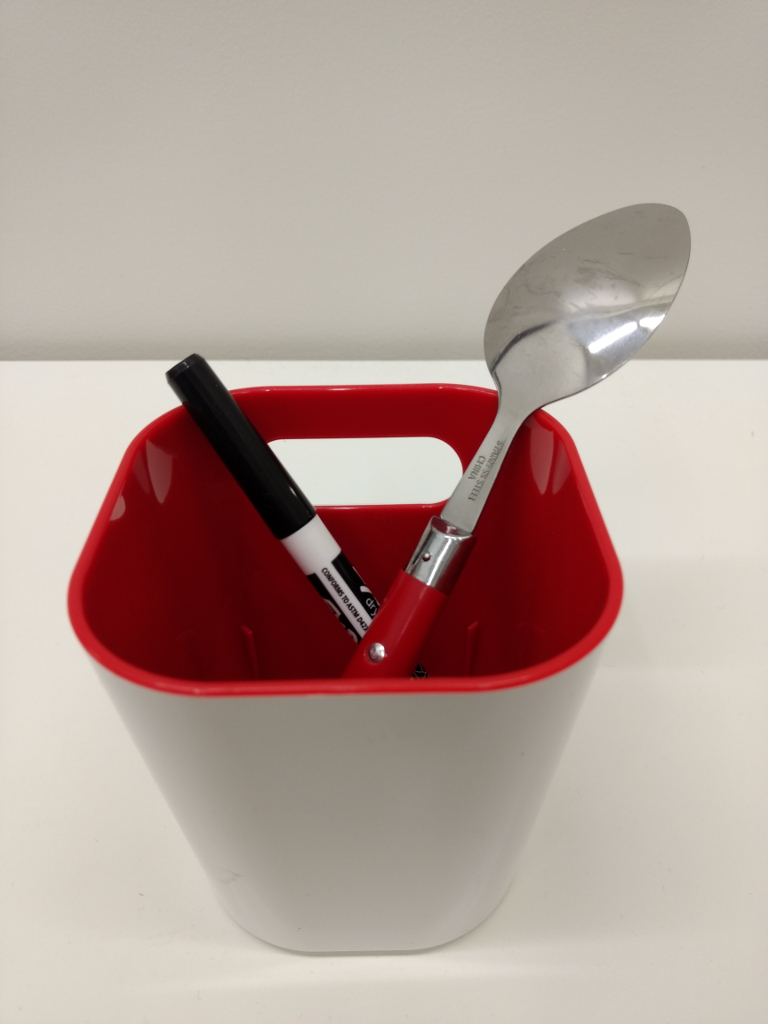
\includegraphics[width=1\textwidth]{{images/orientation_bad_1.jpg}}
  		\caption{}
  		\label{fig:orientationbad1}
	\end{subfigure}
	\caption{Example of a correct a) markers and b) cutlery orientation-based items' delivery, and c) incorrect delivery, where the tips should face downwards.}
	\label{fig:orientation}
\end{figure}

\begin{itemize}
    \item Bonus points can be given if the team opts for the bonus challenges (50 points):
        \SubItem{Opening the three shelf drawers. No further human interaction is allowed. If the robot opens the drawers such that no object can fit in there and therefore the referee or the operator needs to open it more, no bonus points will be considered.}
\end{itemize}

\begin{itemize}
    \item Penalty points in \textbf{Clean Up} can be given in the following scenarios:
        %\SubItem{The robot moves to room 2 before the task is completed (i.e. placing at least one object into their correct location) or the time limit ($\pm$ 15 seconds) is reached: -100 points.}
        \SubItem{Dropping an object (however, if the robot successfully re-takes the same object, no penalisation will be considered): Points x 50\% in the next object.}
        \SubItem{The robot (except for the manipulator's fingers and palm, see Figure \ref{fig:handhitareas}) or the additional equipment prepared by the team hits any object/obstacle inside the arena or in the shelf, or any part of the robot hits the furniture or walls: Points x 50\% for the current object.}
        \SubItem{The robot performs a false delivery (i.e. moves to the deposit location without holding any object in its manipulator): Points x0.0 for the current object.}
\end{itemize}

IMPORTANT: \textbf{Emergency stop.} If the referees or the TC observe behaviours out of the 4S philosophy (Speed, Smooth/Smart, Stable, Safe) such as the robot constantly hitting objects while navigating or grasping objects (i.e. no path and or motion planning is being used), repeatedly dropping objects (i.e. no intelligent manipulation strategies are in use), and so on, they can stop the test and grant zero points for that trial to the team.

\begin{figure}[!h]
\centering
	\begin{subfigure}{.30\textwidth}
  		\centering
  		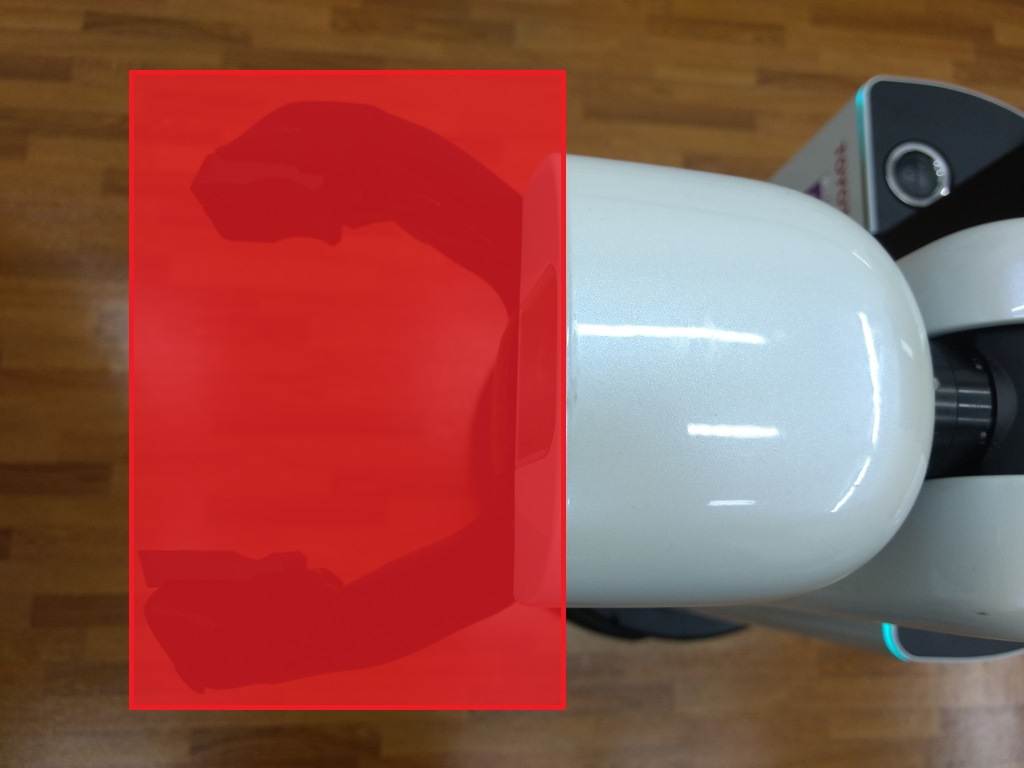
\includegraphics[width=1\textwidth]{{images/hand_a.jpg}}
  		\caption{}
  		\label{fig:handareas}
	\end{subfigure}
	\begin{subfigure}{.30\textwidth}
  		\centering
  		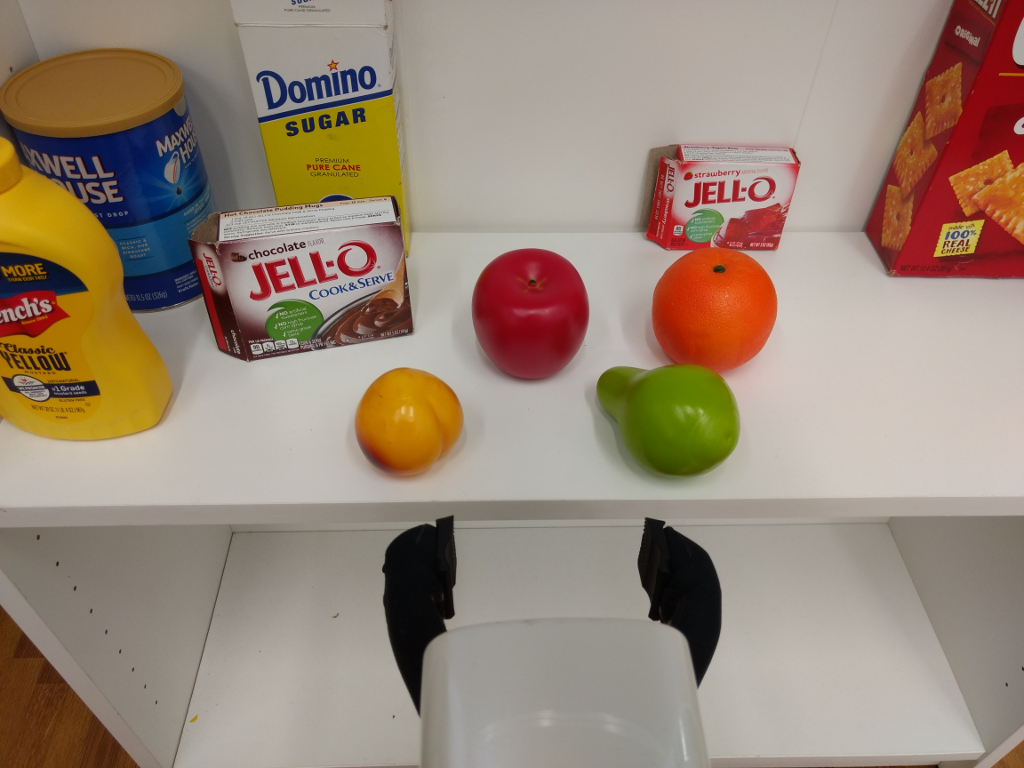
\includegraphics[width=1\textwidth]{{images/hand_b.jpg}}
  		\caption{}
  		\label{fig:handnohit}
	\end{subfigure} \\
	\begin{subfigure}{.30\textwidth}
  		\centering
  		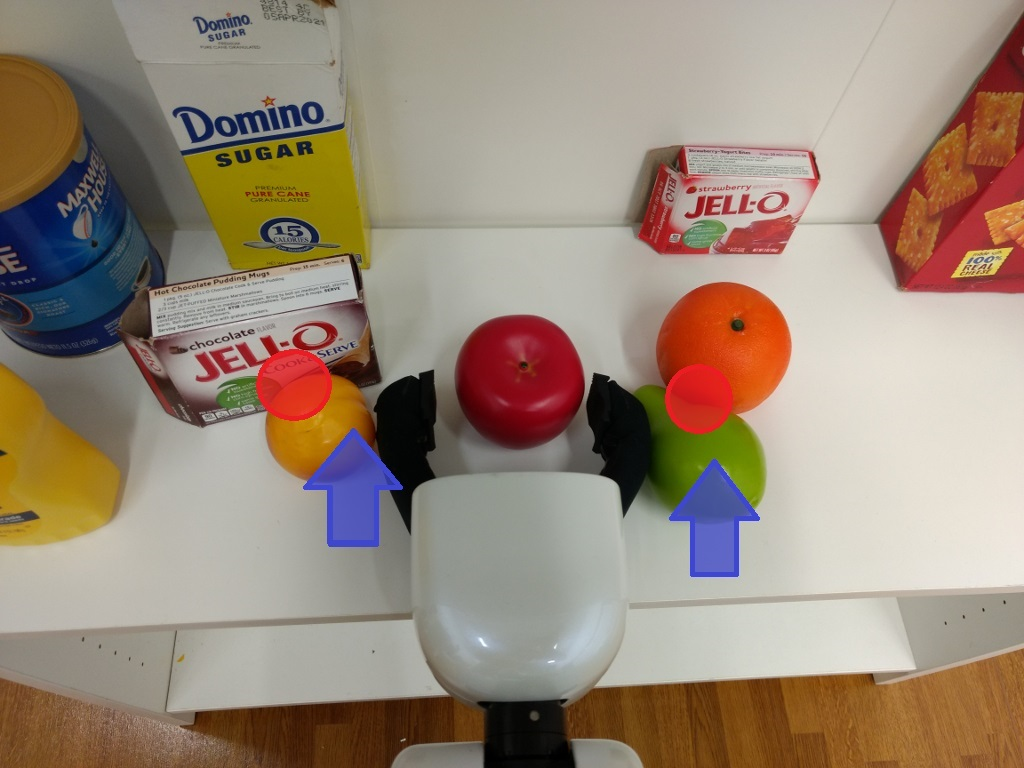
\includegraphics[width=1\textwidth]{{images/hand_c.jpg}}
  		\caption{}
  		\label{fig:handnohitb}
	\end{subfigure}
	\begin{subfigure}{.30\textwidth}
  		\centering
  		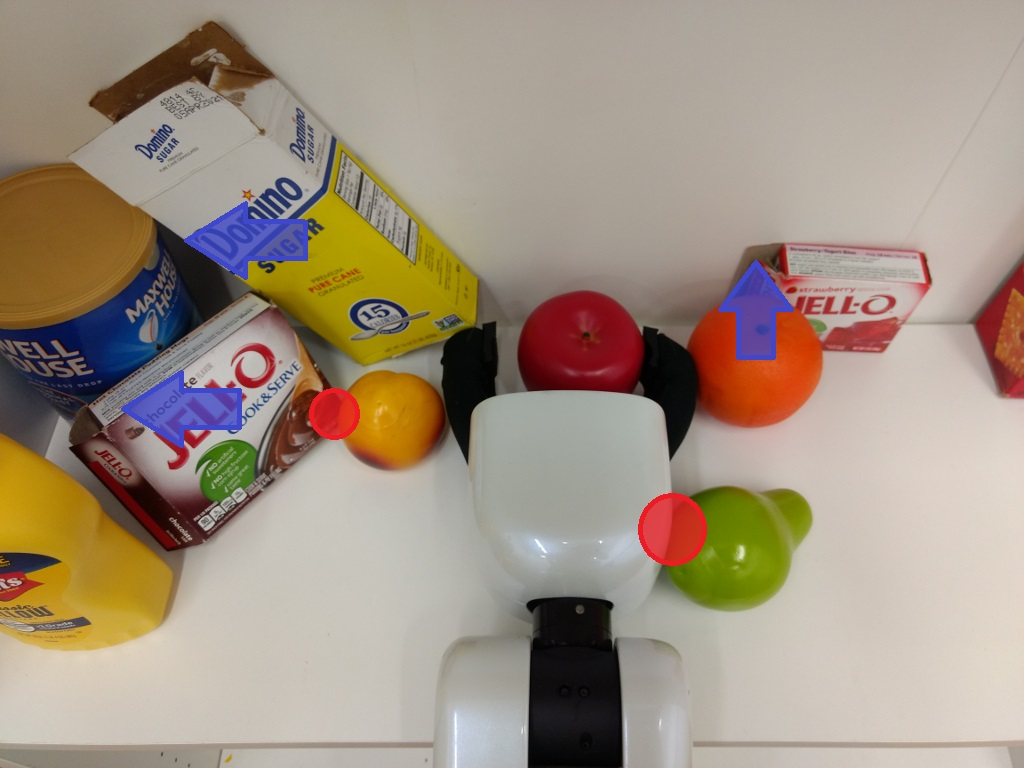
\includegraphics[width=1\textwidth]{{images/hand_d.jpg}}
  		\caption{}
  		\label{fig:handhit}
	\end{subfigure}
	\caption{a) Valid manipulator's fingers and palm areas that can be in contact with an object without being considered a hit. b) In the example, to take the apple surrounded by two objects, c) it is allowed to move the objects around the target object without dropping them or hitting and moving neighbour objects with the displaced objects. d) A hit is considered when the robot hand (except the fingers and palm) or any other part of the robot touches an object (e.g. the pear in the image) or when the center of mass of a neighbour object is displaced two or more centimeters after a hit by a displaced object (e.g. the boxes were significantly moved after a hit by the peach).}
	\label{fig:handhitareas} 
\end{figure}

\clearpage
\subsection{Go and Get It}

\textbf{Description:} Provide a person with something to consume when requested.
\textbf{Time:} 5 min for Stage I

\subsubsection{Settings}

\noindent
\textbf{Environment}
\begin{itemize}
    \item The robot starts at the front entrance; the robot reads what object to deliver.
    \item Furniture: shelf without door (Figure \ref{fig:shelf}), chair (x2).
    \item Storage places: shelf without door.
\end{itemize}

\begin{figure}[!h]
	\centering
	%\begin{subfigure}{.45\textwidth}
  		%\centering
  		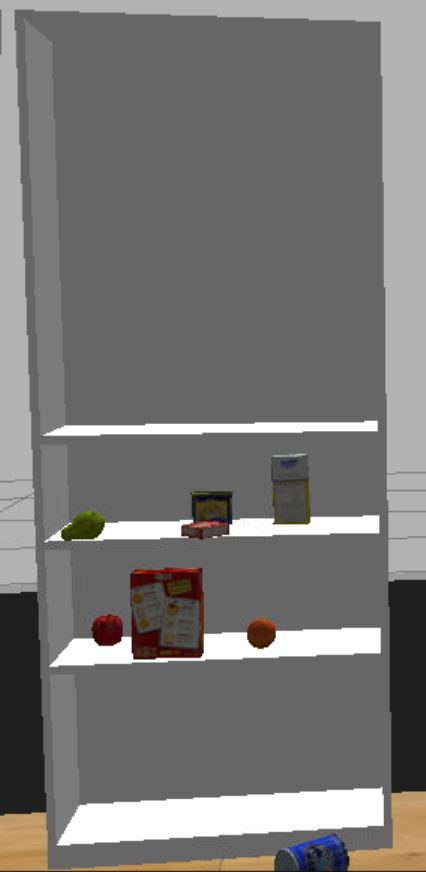
\includegraphics[width=0.45\textwidth]{{images/shelf.jpg}}
  		%\caption{}
  		%\label{fig:objects}
	%\end{subfigure}
	%\begin{subfigure}{.45\textwidth}
  	%	\centering
  	%	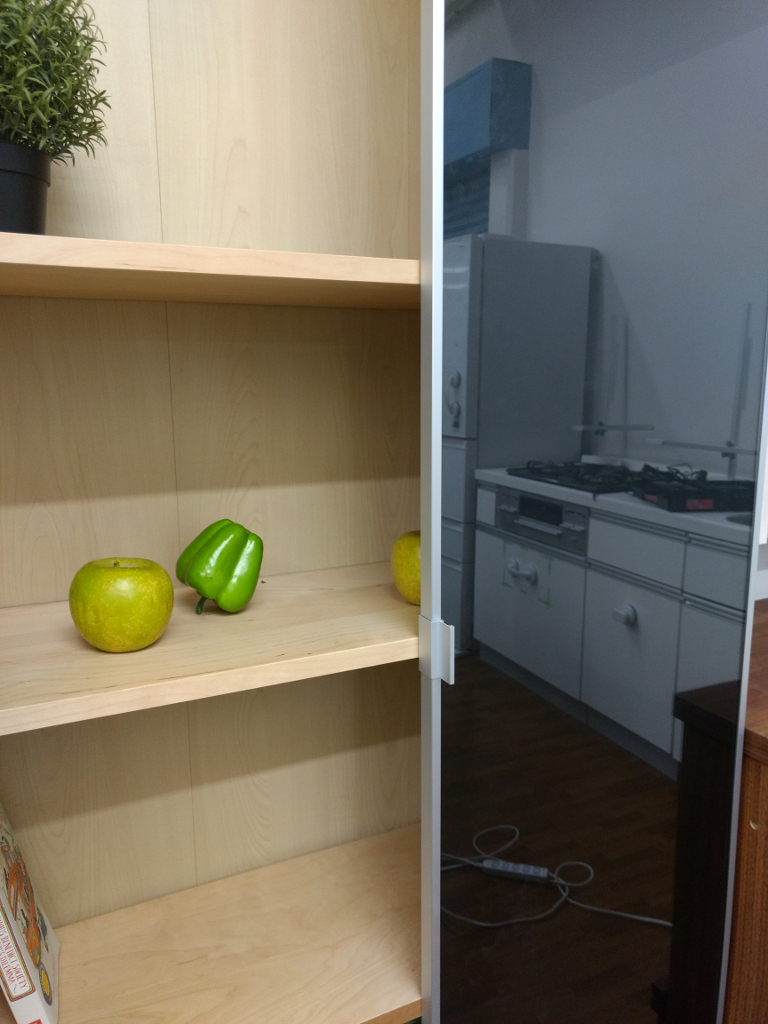
\includegraphics[width=1\textwidth]{{images/lateral_door_b.jpg}}
  	%	\caption{}
  	%	\label{fig:door}
	%\end{subfigure}
	\caption{Front view of the shelf and objects inside it.}
	\label{fig:shelf}
\end{figure}

\noindent
\textbf{Task Performance}
\begin{itemize}
    \item The robot starts at the front entrance; there might be objects on the floor of Room I according to the Clean Up regulations (i.e. same initial setup for all the competition).
    \item The location of the shelf is known and fixed.
\end{itemize}

\subsubsection{Before the Competition}

\begin{itemize}
    \item Teams are given the time to create/adjust map data in the actual apartment.
    \item Right before the competition, the referee sets the rooms into messy condition (within a specified error tolerance range).
    \item Room 1. Living room (task planning, object recognition and manipulation), as a default setup:
        \SubItem{30 objects (5 categories, 5 known + 1 unknown objects per category) are randomly placed in the room (on the floor and or tables).}
    \item Room 2. Dining space (HRI, path and motion planning), for the Go and Get It task:
        \SubItem{Obstacles on the floor are set in the access between rooms. Several food items are placed inside the shelf. Some people are in the dining room.}
\end{itemize}

\subsubsection{During the Competition}

The robot enters the living room in a messy condition. Three runs are allowed per trial. A detailed description of a full run is described bellow:

\begin{itemize}
    \item Each test starts with the robot at the front entrance (starting point). The start signal is the robot motion.
    \item Task 2a
        \SubItem{Enters the dining room and goes to a location inside the room while avoiding obstacles.}
    \item Task 2b
        \SubItem{The robot goes directly to the shelf and takes the correct object given at the beginning of the test.}
        \SubItem{The robot moves toward the group of persons and gives the object to the one requesting it.}
        \SubItem{The test ends with the robot reporting the completion of the task or the time is over.}
\end{itemize}

In the simulator, there will be a delivery area, as in Figure \ref{fig:arenaareas}, and it will be divided into left and right side. A person will be randomly located in each side, and within a reachable position to the robot; they will be reffered as "left person" and "right person".

Commands are provided to the robot trough the \textbf{/message} topic as follows:

\begin{itemize}
    \item When robot enters Room 2 The target object is published.
    \item When robot enters the delivery area: The target person is published.
    \item When robot approaches a person: A "done" message is published.
\end{itemize}

\subsubsection{Scores} \label{sec:scores}

\begin{itemize}
    \item Task 2a
        \SubItem{Navigating to a location in Room 2 while avoiding random obstacles lying on the floor within the access area. As we are considering very small and flat objects, a collision will be reckoned if there is physical contact with any object on the floor: 100 points.}
    \item Task 2b
        \SubItem{Grasping any food item in the shelf: 30 points x 1 unit.}
        \SubItem{Correctly taking the requested food item among many objects in the shelf: 70 additional points. Note that the requested object is likely to be occluded by other items in the shelf and therefore a grasping strategy should be implemented (e.g. first move item one and item two in front of the target object and without hitting any other object in the shelf before being able to take the requested object).}
        \SubItem{Delivering the object to a person in the delivery area: 30 points x 1 person.}
        \SubItem{Correctly detecting a person request and giving the food item to her/him: 70 additional points.}
        \SubItem{Correctly finishing the task within time limit (i.e. correct object delivered to the right person and without collisions): 50 points.}
        \SubItem{If any time remaining, add 20 points per minute.}
    \item The best execution (highest scored run) will be taken as score for that particular trial.
\end{itemize}

\begin{itemize}
    \item Penalty points in \textbf{Go and Get It} are considered in the following scenarios:
        \SubItem{Dropping an object out of the shelf (however, if the robot successfully re-takes the same object and delivers it back inside the shelf, no penalisation will be considered): 0.25 x Partial points in Task 2b$_1$ (considered as a HIT in the score sheet).}
        \SubItem{The robot (except for the manipulator's fingers and palm, see Figure \ref{fig:handhitareas}) or the additional equipment prepared by the team hits any object/obstacle inside the arena or in the shelf, or any part of the robot hits the furniture or walls: 0.25 x Partial points in Task 2b$_1$ or Task 2b$_2$ (considered as a HIT in the score sheet).}
        \SubItem{The robot performs a false delivery (i.e. moves to the deposit location without holding any object in its manipulator): Points x0.0 in Task 2b.}
\end{itemize}

IMPORTANT: \textbf{Emergency stop.} If the referees or the TC observe behaviours out of the 4S philosophy (Speed, Smooth/Smart, Stable, Safe) such as the robot constantly hitting objects while navigating or grasping objects (i.e. no path and or motion planning is being used), repeatedly dropping objects (i.e. no intelligent manipulation strategies are in use), and so on, they can stop the test and grant zero points for that trial to the team.

\clearpage
\subsection{Additional rules and remarks}

\begin{itemize}
    \item The robot can use any type of external computing (e.g. cloud computing) and can connect to it via wireless (WiFi provided, but not guaranteed).
    \item Random robot inspections will be performed during the competition.
\end{itemize}

IMPORTANT: \textbf{External devices notification.} Before using external tools or performing any hardware modification, teams should submit to the committee a letter of intent specifying the details of such tool or modification to receive approval and or feedback.

\subsection{Special considerations}

The core task in this test is having a robot that autonomously tidies up a messed room as a human would do. 

This rulebook presents a series of guidelines and regulations that objectively allows evaluating the different aspects of the 4S philosophy (Speed, Smooth/Smart, Stable, Safe) and therefore the expected behaviour of a robot is not limited to the rules established here. 

In principle, any robot behaviour not regulated here is allowed as long as it doesn't interfere with solving the core task. However, the Technical Committee is allowed to ban any behaviour not mentioned here and that they may consider unfair (e.g. taking several objects at the same time without announcing it and without a clear object recognition; asking for human interaction beyond the established in the rulebook; etc). If you have any concern about a behaviour that may seem controversial, please contact the TC before considering their application to solving the task.

\iffalse
\clearpage
%\pagebreak
\subsection{Score Sheet}

Total score per match:

%\begin{table}
\begin{center}
\begin{tabular}{ |m{8cm}|m{3cm}|m{1cm}| } 
    \hline
    \textbf{Performance} & \textbf{Score} & \textbf{Points} \\ 
    \hline
    \textbf{\textit{Task 1}} & & \\ 
    \hline
    Grasping an object inside the room & 10 x 30 & \\ 
    \hline
    Correctly depositing an object in a location & 10 x 30 & \\ 
    \hline
    Correctly depositing an object in a location according to its category & +10 per object & \\ 
    \hline
    Correctly depositing an object based on its orientation (e.g. cups facing upwards, pencil tips facing downwards) & +10 per object & \\
    \hline
    Finishing the task within the time limit (15 min $\pm$ 15 sec) & 50 points & \\ 
    \hline
    & & \\ 
    \hline
    \textbf{\textit{Task 2a}} & & \\ 
    \hline
    Successfully entering the arena without collisions & 100 & \\ 
    \hline
    Hitting an obstacle & -50 per hit & \\ 
    \hline
    \textbf{\textit{Task 2b}} & & \\ 
    \hline
    Taking the target object among many objects in the shelf & 100 & \\ 
    \hline
    Taking the wrong object & -70 & \\ 
    \hline
    Correctly detecting a person request and giving the drink to her/him & 100 & \\ 
    \hline
    Delivering the object to the wrong person & -70 & \\ 
    \hline
    Finishing the task within time limit (5 min $\pm$ 15 sec) & 50 & \\ 
    \hline
     & & \\ 
    \hline
    \textbf{\textit{Special Bonuses}} & & \\ 
    \hline
    If any time remaining, add 1 points per minute & 20 x time & \\ 
    \hline
    Bonus challenges (Hard-to-grasp object manipulation, Opening the three drawers) & 50 per challenge & \\ 
    \hline
    \textbf{\textit{Penalties}} & & \\ 
    \hline
    Moving to the next room before time & -100 & \\ 
    \hline
    Hitting the furniture or the objects/obstacles inside the arena & -50 per hit & \\ 
    \hline
    Dropping an object without re-taking it & -10 per object & \\ 
    \hline
    Performing a false delivery & -10 per delivery & \\ 
    \hline
    Restart (within one minute) & -100 & \\ 
    \hline
    Additional restarting time & -100 per minute & \\ 
    \hline
    \hline
    \textbf{Total (no penalties/bonuses considered)} & & 1000 \\ 
    \hline
\end{tabular}
\end{center}
%\label{table:scores}
%\end{table}
\fi

\clearpage
%\pagebreak
\subsection{Score Sheet - Clean Up}

Total score per match:\\ \\

\begin{center} Team name/number: $\rule{6cm}{0.15mm}$ \end{center}

%\begin{table}
\begin{center}
\begin{tabular}{|m{0.4cm}|m{0.8cm}|m{1.2cm}|m{1cm}|m{1cm}|m{0.8cm}|m{0.8cm}|m{1cm}|m{0.8cm}|m{0.8cm}|}
    \hline
    &\multicolumn{4}{|c|}{Penalties }& \multicolumn{5}{|c|}{Points }\\
    \cline{2-10}
    & & &\multicolumn{2}{|c|}{Hit}&\multicolumn{3}{|c|}{Correct}& &\\
    \cline{4-5} \cline{6-8}
    \#& Drop& Restart& Object& Furni- ture& Deli- very& Cate- gory& Orien- tation& False& Total \\
    \hline
     & \multicolumn{1}{|c|}{x0.5} & \multicolumn{1}{|c|}{x0.5} & \multicolumn{1}{|c|}{x0.5} & \multicolumn{1}{|c|}{x0.5}& 10& +10& +10& x0.0&\\
    \cline{2-9}
    1 & \multicolumn{8}{|l|}{Notes: }&\\
    \hline
     & \multicolumn{1}{|c|}{x0.5} & \multicolumn{1}{|c|}{x0.5} & \multicolumn{1}{|c|}{x0.5} & \multicolumn{1}{|c|}{x0.5}& 10& +10& +10& x0.0&\\
    \cline{2-9}
    2 & \multicolumn{8}{|l|}{Notes: }&\\
    \hline
     & \multicolumn{1}{|c|}{x0.5} & \multicolumn{1}{|c|}{x0.5} & \multicolumn{1}{|c|}{x0.5} & \multicolumn{1}{|c|}{x0.5}& 10& +10& +10& x0.0&\\
    \cline{2-9}
    3 & \multicolumn{8}{|l|}{Notes: }&\\
    \hline
     & \multicolumn{1}{|c|}{x0.5} & \multicolumn{1}{|c|}{x0.5} & \multicolumn{1}{|c|}{x0.5} & \multicolumn{1}{|c|}{x0.5}& 10& +10& +10& x0.0&\\
    \cline{2-9}
    4 & \multicolumn{8}{|l|}{Notes: }&\\
    \hline
     & \multicolumn{1}{|c|}{x0.5} & \multicolumn{1}{|c|}{x0.5} & \multicolumn{1}{|c|}{x0.5} & \multicolumn{1}{|c|}{x0.5}& 10& +10& +10& x0.0&\\
    \cline{2-9}
    5 & \multicolumn{8}{|l|}{Notes: }&\\
    \hline
     & \multicolumn{1}{|c|}{x0.5} & \multicolumn{1}{|c|}{x0.5} & \multicolumn{1}{|c|}{x0.5} & \multicolumn{1}{|c|}{x0.5}& 10& +10& +10& x0.0&\\
    \cline{2-9}
    6 & \multicolumn{8}{|l|}{Notes: }&\\
    \hline
     & \multicolumn{1}{|c|}{x0.5} & \multicolumn{1}{|c|}{x0.5} & \multicolumn{1}{|c|}{x0.5} & \multicolumn{1}{|c|}{x0.5}& 10& +10& +10& x0.0&\\
    \cline{2-9}
    7 & \multicolumn{8}{|l|}{Notes: }&\\
    \hline
     & \multicolumn{1}{|c|}{x0.5} & \multicolumn{1}{|c|}{x0.5} & \multicolumn{1}{|c|}{x0.5} & \multicolumn{1}{|c|}{x0.5}& 10& +10& +10& x0.0&\\
    \cline{2-9}
    8 & \multicolumn{8}{|l|}{Notes: }&\\
    \hline
     & \multicolumn{1}{|c|}{x0.5} & \multicolumn{1}{|c|}{x0.5} & \multicolumn{1}{|c|}{x0.5} & \multicolumn{1}{|c|}{x0.5}& 10& +10& +10& x0.0&\\
    \cline{2-9}
    9 & \multicolumn{8}{|l|}{Notes: }&\\
    \hline
     & \multicolumn{1}{|c|}{x0.5} & \multicolumn{1}{|c|}{x0.5} & \multicolumn{1}{|c|}{x0.5} & \multicolumn{1}{|c|}{x0.5}& 10& +10& +10& x0.0&\\
    \cline{2-9}
    10 & \multicolumn{8}{|l|}{Notes: }&\\
    \hline
     & \multicolumn{1}{|c|}{x0.5} & \multicolumn{1}{|c|}{x0.5} & \multicolumn{1}{|c|}{x0.5} & \multicolumn{1}{|c|}{x0.5}& 10& +10& +10& x0.0&\\
    \cline{2-9}
    11 & \multicolumn{8}{|l|}{Notes: }&\\
    \hline
     & \multicolumn{1}{|c|}{x0.5} & \multicolumn{1}{|c|}{x0.5} & \multicolumn{1}{|c|}{x0.5} & \multicolumn{1}{|c|}{x0.5}& 10& +10& +10& x0.0&\\
    \cline{2-9}
    12 & \multicolumn{8}{|l|}{Notes: }&\\
    \hline
     & \multicolumn{1}{|c|}{x0.5} & \multicolumn{1}{|c|}{x0.5} & \multicolumn{1}{|c|}{x0.5} & \multicolumn{1}{|c|}{x0.5}& 10& +10& +10& x0.0&\\
    \cline{2-9}
    13 & \multicolumn{8}{|l|}{Notes: }&\\
    \hline
     & \multicolumn{1}{|c|}{x0.5} & \multicolumn{1}{|c|}{x0.5} & \multicolumn{1}{|c|}{x0.5} & \multicolumn{1}{|c|}{x0.5}& 10& +10& +10& x0.0&\\
    \cline{2-9}
    14 & \multicolumn{8}{|l|}{Notes: }&\\
    \hline
     & \multicolumn{1}{|c|}{x0.5} & \multicolumn{1}{|c|}{x0.5} & \multicolumn{1}{|c|}{x0.5} & \multicolumn{1}{|c|}{x0.5}& 10& +10& +10& x0.0&\\
    \cline{2-9}
    15 & \multicolumn{8}{|l|}{Notes: }&\\
    \hline
    \multicolumn{10}{|l|}{Comments:} \\ 
    \multicolumn{10}{|l|}{} \\
    \multicolumn{10}{|l|}{} \\
    \hline
\end{tabular}
\end{center}
%\label{table:scores}
%\end{table}

\clearpage

%\begin{table}
\begin{center}
\begin{tabular}{|m{0.4cm}|m{0.8cm}|m{1cm}|m{1cm}|m{1.2cm}|m{0.8cm}|m{0.8cm}|m{1cm}|m{0.8cm}|m{0.8cm}|}
    \hline
    &\multicolumn{4}{|c|}{Penalties }& \multicolumn{5}{|c|}{Points }\\
    \cline{2-10}
    & & &\multicolumn{2}{|c|}{Hit}&\multicolumn{3}{|c|}{Correct}& &\\
    \cline{4-5} \cline{6-8}
    \#& Drop& Restart& Object& Furni- ture& Deli- very& Cate- gory& Orien- tation& False& Total \\
    \hline
     & \multicolumn{1}{|c|}{x0.5} & \multicolumn{1}{|c|}{x0.5} & \multicolumn{1}{|c|}{x0.5} & \multicolumn{1}{|c|}{x0.5}& 10& +10& +10& x0.0&\\
    \cline{2-9}
    16 & \multicolumn{8}{|l|}{Notes: }&\\
    \hline
     & \multicolumn{1}{|c|}{x0.5} & \multicolumn{1}{|c|}{x0.5} & \multicolumn{1}{|c|}{x0.5} & \multicolumn{1}{|c|}{x0.5}& 10& +10& +10& x0.0&\\
    \cline{2-9}
    17 & \multicolumn{8}{|l|}{Notes: }&\\
    \hline
     & \multicolumn{1}{|c|}{x0.5} & \multicolumn{1}{|c|}{x0.5} & \multicolumn{1}{|c|}{x0.5} & \multicolumn{1}{|c|}{x0.5}& 10& +10& +10& x0.0&\\
    \cline{2-9}
    18 & \multicolumn{8}{|l|}{Notes: }&\\
    \hline
     & \multicolumn{1}{|c|}{x0.5} & \multicolumn{1}{|c|}{x0.5} & \multicolumn{1}{|c|}{x0.5} & \multicolumn{1}{|c|}{x0.5}& 10& +10& +10& x0.0&\\
    \cline{2-9}
    19 & \multicolumn{8}{|l|}{Notes: }&\\
    \hline
     & \multicolumn{1}{|c|}{x0.5} & \multicolumn{1}{|c|}{x0.5} & \multicolumn{1}{|c|}{x0.5} & \multicolumn{1}{|c|}{x0.5}& 10& +10& +10& x0.0&\\
    \cline{2-9}
    20 & \multicolumn{8}{|l|}{Notes: }&\\
    \hline
     & \multicolumn{1}{|c|}{x0.5} & \multicolumn{1}{|c|}{x0.5} & \multicolumn{1}{|c|}{x0.5} & \multicolumn{1}{|c|}{x0.5}& 10& +10& +10& x0.0&\\
    \cline{2-9}
    21 & \multicolumn{8}{|l|}{Notes: }&\\
    \hline
     & \multicolumn{1}{|c|}{x0.5} & \multicolumn{1}{|c|}{x0.5} & \multicolumn{1}{|c|}{x0.5} & \multicolumn{1}{|c|}{x0.5}& 10& +10& +10& x0.0&\\
    \cline{2-9}
    22 & \multicolumn{8}{|l|}{Notes: }&\\
    \hline
     & \multicolumn{1}{|c|}{x0.5} & \multicolumn{1}{|c|}{x0.5} & \multicolumn{1}{|c|}{x0.5} & \multicolumn{1}{|c|}{x0.5}& 10& +10& +10& x0.0&\\
    \cline{2-9}
    23 & \multicolumn{8}{|l|}{Notes: }&\\
    \hline
     & \multicolumn{1}{|c|}{x0.5} & \multicolumn{1}{|c|}{x0.5} & \multicolumn{1}{|c|}{x0.5} & \multicolumn{1}{|c|}{x0.5}& 10& +10& +10& x0.0&\\
    \cline{2-9}
    24 & \multicolumn{8}{|l|}{Notes: }&\\
    \hline
     & \multicolumn{1}{|c|}{x0.5} & \multicolumn{1}{|c|}{x0.5} & \multicolumn{1}{|c|}{x0.5} & \multicolumn{1}{|c|}{x0.5}& 10& +10& +10& x0.0&\\
    \cline{2-9}
    25 & \multicolumn{8}{|l|}{Notes: }&\\
    \hline
     & \multicolumn{1}{|c|}{x0.5} & \multicolumn{1}{|c|}{x0.5} & \multicolumn{1}{|c|}{x0.5} & \multicolumn{1}{|c|}{x0.5}& 10& +10& +10& x0.0&\\
    \cline{2-9}
    26 & \multicolumn{8}{|l|}{Notes: }&\\
    \hline
     & \multicolumn{1}{|c|}{x0.5} & \multicolumn{1}{|c|}{x0.5} & \multicolumn{1}{|c|}{x0.5} & \multicolumn{1}{|c|}{x0.5}& 10& +10& +10& x0.0&\\
    \cline{2-9}
    27 & \multicolumn{8}{|l|}{Notes: }&\\
    \hline
     & \multicolumn{1}{|c|}{x0.5} & \multicolumn{1}{|c|}{x0.5} & \multicolumn{1}{|c|}{x0.5} & \multicolumn{1}{|c|}{x0.5}& 10& +10& +10& x0.0&\\
    \cline{2-9}
    28 & \multicolumn{8}{|l|}{Notes: }&\\
    \hline
     & \multicolumn{1}{|c|}{x0.5} & \multicolumn{1}{|c|}{x0.5} & \multicolumn{1}{|c|}{x0.5} & \multicolumn{1}{|c|}{x0.5}& 10& +10& +10& x0.0&\\
    \cline{2-9}
    29 & \multicolumn{8}{|l|}{Notes: }&\\
    \hline
     & \multicolumn{1}{|c|}{x0.5} & \multicolumn{1}{|c|}{x0.5} & \multicolumn{1}{|c|}{x0.5} & \multicolumn{1}{|c|}{x0.5}& 10& +10& +10& x0.0&\\
    \cline{2-9}
    30 & \multicolumn{8}{|l|}{Notes: }&\\
    \hline
    \multicolumn{9}{|l|}{Finishing the task within the time limit (15 min $\pm$ 15 sec): 50 points} & \\
    \hline
    \multicolumn{9}{|l|}{Bonus challenges (50 points):} &\\
    \multicolumn{9}{|l|}{--Opening the three drawers (without further human interaction)} &\\
    \hline
    \multicolumn{9}{|r|}{\textbf{TOTAL (Clean Up)}  } &\\ 
    \hline
    \multicolumn{10}{|l|}{Comments:} \\ 
    \multicolumn{10}{|l|}{} \\
    \multicolumn{10}{|l|}{} \\
    \hline
\end{tabular}
\end{center}
%\label{table:scores}
%\end{table}

\begin{center} Referee: $\rule{3cm}{0.15mm}$ Team Leader: $\rule{3cm}{0.15mm}$ \end{center}

\clearpage
%\pagebreak

\subsection{Score Sheet - Go and Get It}

Total score per match:\\ \\

\begin{center} Team name/number: $\rule{6cm}{0.15mm}$ \end{center}

%\begin{table}
\begin{center}
\begin{tabular}{ |m{8cm}|m{3cm}|m{1cm}| } 
    \hline
    \multicolumn{3}{|l|}{\textbf{\textit{Task 2a}}} \\ 
    \hline
    Successfully entering to the dining room without collisions & 100 & \\ 
    \hline
    \multicolumn{3}{|l|}{\textbf{\textit{Task 2b}}} \\ 
    \hline
    Taking any food item in the shelf & 40 & \\ 
    \hline
    Taking the requested object among many objects in the shelf & +60 & \\ 
    \hline
    \multicolumn{2}{|r|}{SUM$_1$  } &\\
    \hline
    \multicolumn{3}{|l|}{HIT$_1$:\hspace*{2cm} 1\hspace*{2cm} 2\hspace*{2cm} 3\hspace*{2cm} 4+} \\ 
    \hline
    \multicolumn{2}{|r|}{Task\_2b$_1$ = (1 - 0.25xHIT$_1$)xSUM$_1$} &\\
    \hline
    \multicolumn{3}{|l|}{}\\
    \hline
    Delivering the object to a person in the delivery area & 40 & \\ 
    \hline
    Correctly detecting a person's request and giving the item to her/him & +60 & \\ 
    \hline
    \multicolumn{2}{|r|}{SUM$_2$  } &\\
    \hline
    \multicolumn{3}{|l|}{HIT$_2$:\hspace*{2cm} 1\hspace*{2cm} 2\hspace*{2cm} 3\hspace*{2cm} 4+} \\ 
    \hline
    \multicolumn{2}{|r|}{Task\_2b$_2$ = (1 - 0.25xHIT$_2$)xSUM$_2$} &\\
    \hline
    \multicolumn{3}{|l|}{}\\
    \hline
    \multicolumn{2}{|r|}{SUM = Task\_2a + Task\_2b$_1$ + Task\_2b$_2$  } &\\
    \hline
    \multicolumn{3}{|l|}{}\\
    \hline
    Finishing the task within the time limit (5 min $\pm$ 15 sec) & 50 & \\ 
    \hline
    If any time remaining, add 20 points per minute & 20 x minutes & \\ 
    \hline
    \multicolumn{2}{|r|}{\textbf{TOTAL (Go and Get It)}  } &\\
    \hline
\end{tabular}
\end{center}

\begin{center}
\begin{tabular}{ |m{8cm}|m{3cm}|m{1cm}| } 
    \hline
    \multicolumn{3}{|l|}{\textbf{\textit{Special Penalties}}  (Clean Up and Go and Get It)} \\ 
    \hline
    Emergency stop by a referee & Total points x 0.0 & \\
    \hline
    \multicolumn{3}{|l|}{}\\
    \hline
    \multicolumn{3}{|l|}{Note: a HIT considers dropping an object out of the shelf, a restart,} \\
    \multicolumn{3}{|l|}{and a regular collision.} \\ 
    \hline
\end{tabular}
\end{center}
%\label{table:scores}
%\end{table}

\begin{center} Referee: $\rule{3cm}{0.15mm}$ Team Leader: $\rule{3cm}{0.15mm}$ \end{center}

\clearpage
\section{Appendix}
\subsection{Furniture models} \label{sec:furniture}

Note: units are in meters in the following order:  width x length x height.

\begin{itemize}
    \item stairs-like drawer (white structure, orange drawers):
    
    Link: \url{https://www.ikea.com/us/en/catalog/products/S89857541/#/S59128935}

    \item long table (white):

    Link: \url{https://www.ikea.com/us/en/catalog/products/00342640/}

    \item tall table (white):

    Link: \url{https://www.ikea.com/us/en/catalog/products/20342644/#/60342642}

    \item bin (two bins, one green and the other black):

    Link: \url{https://www.ikea.com/us/en/catalog/products/10300319/}

    \item  shelf (white):

    Link: \url{https://www.ikea.com/us/en/catalog/products/00263850/}

    \item chair (white structure, gray cover):

    Link: \url{https://www.ikea.com/us/en/catalog/products/S69100163/}
\end{itemize}

\begin{table}[h!]
\begin{center}
\begin{tabular}{ |M{2.0cm}|M{2.0cm}|M{1.0cm}|M{1.0cm}|M{1.0cm}|M{1.5cm}| }
    \hline
    Name & IKEA's Model & width & length & height & Image\\
    \hline
    stairs-like drawer & 591.289.35 & 0.44m & 0.99m & 0.94m & Figure \ref{fig:drawermodel}\\
    \hline
    long table & 003.426.40 & 0.40m & 1.20m & 0.40m & Figure \ref{fig:longtablemodel}\\
    \hline
    tall table & 603.426.42 & 0.40m & 0.40m & 0.60m & Figure \ref{fig:talltablemodel}\\
    \hline
    bin & 103.003.19 & 0.38m & 0.33m & 0.33m & Figure \ref{fig:binmodel}\\
    \hline
    shelf & 002.638.50 & 0.28m & 0.80m & 2.02m & Figure \ref{fig:shelfmodel}\\
    \hline
    chair & 691.001.63 & 0.58m & 0.54m & 0.97m & Figure \ref{fig:chairmodel}\\
    \hline
\end{tabular}
\end{center}
\caption{Furniture's model and size to be used during the tests and competition.}
\label{table:furniture}
\end{table}

\clearpage

\begin{figure}[!h]
  	\centering
  	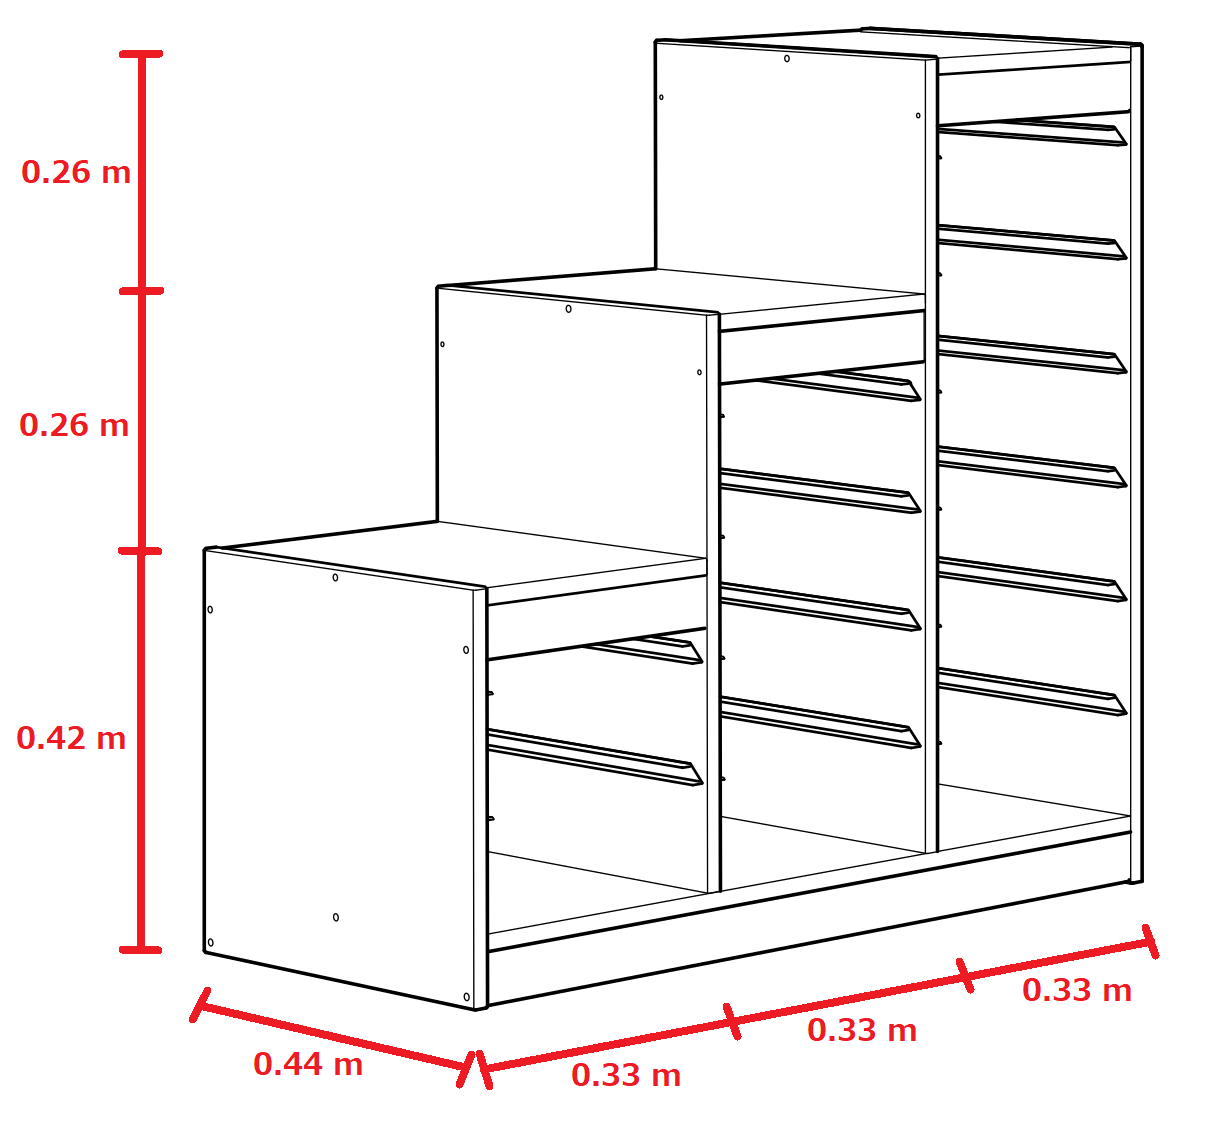
\includegraphics[width=0.80\textwidth]{{images/model_drawer.png}}
	\caption{Stairs-like drawer model (width 0.44 m, length 0.99 m, height 0.94 m).}
	\label{fig:drawermodel}
\end{figure}

\begin{figure}[!h]
  	\centering
  	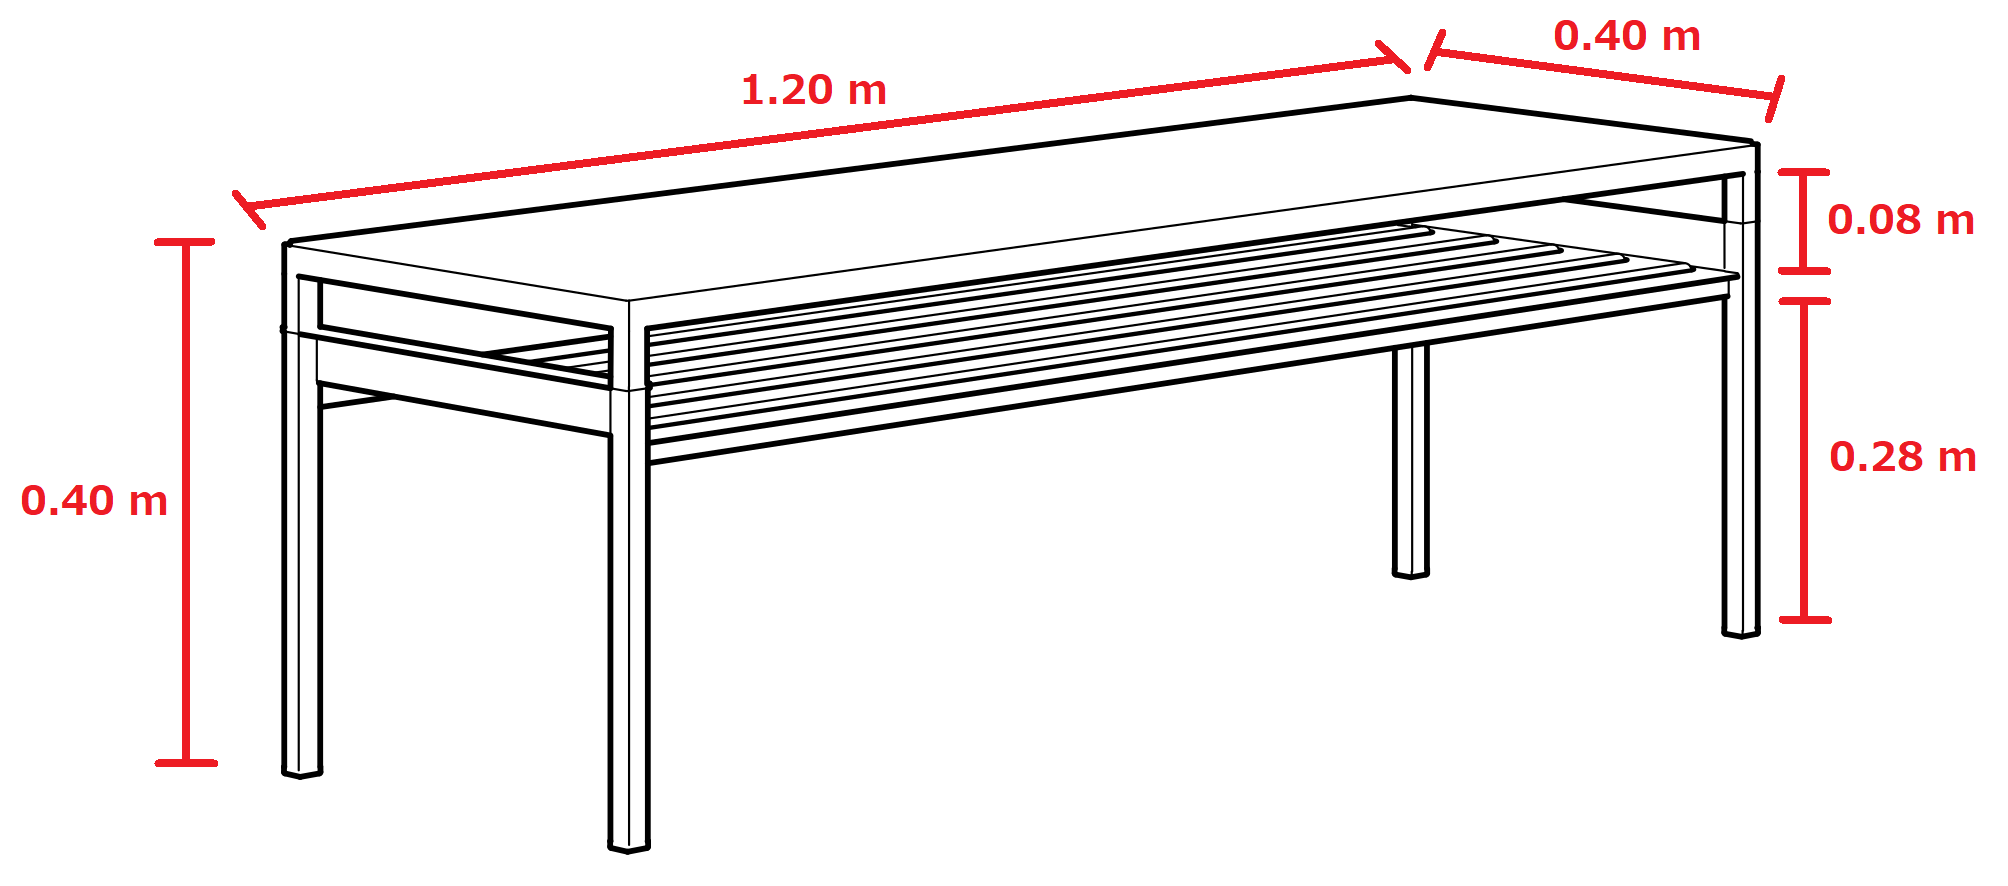
\includegraphics[width=0.80\textwidth]{{images/model_longtable.png}}
	\caption{Long table model (width 0.40, length 1.20, height 0.40 m).}
	\label{fig:longtablemodel}
\end{figure}

\begin{figure}[!h]
  	\centering
  	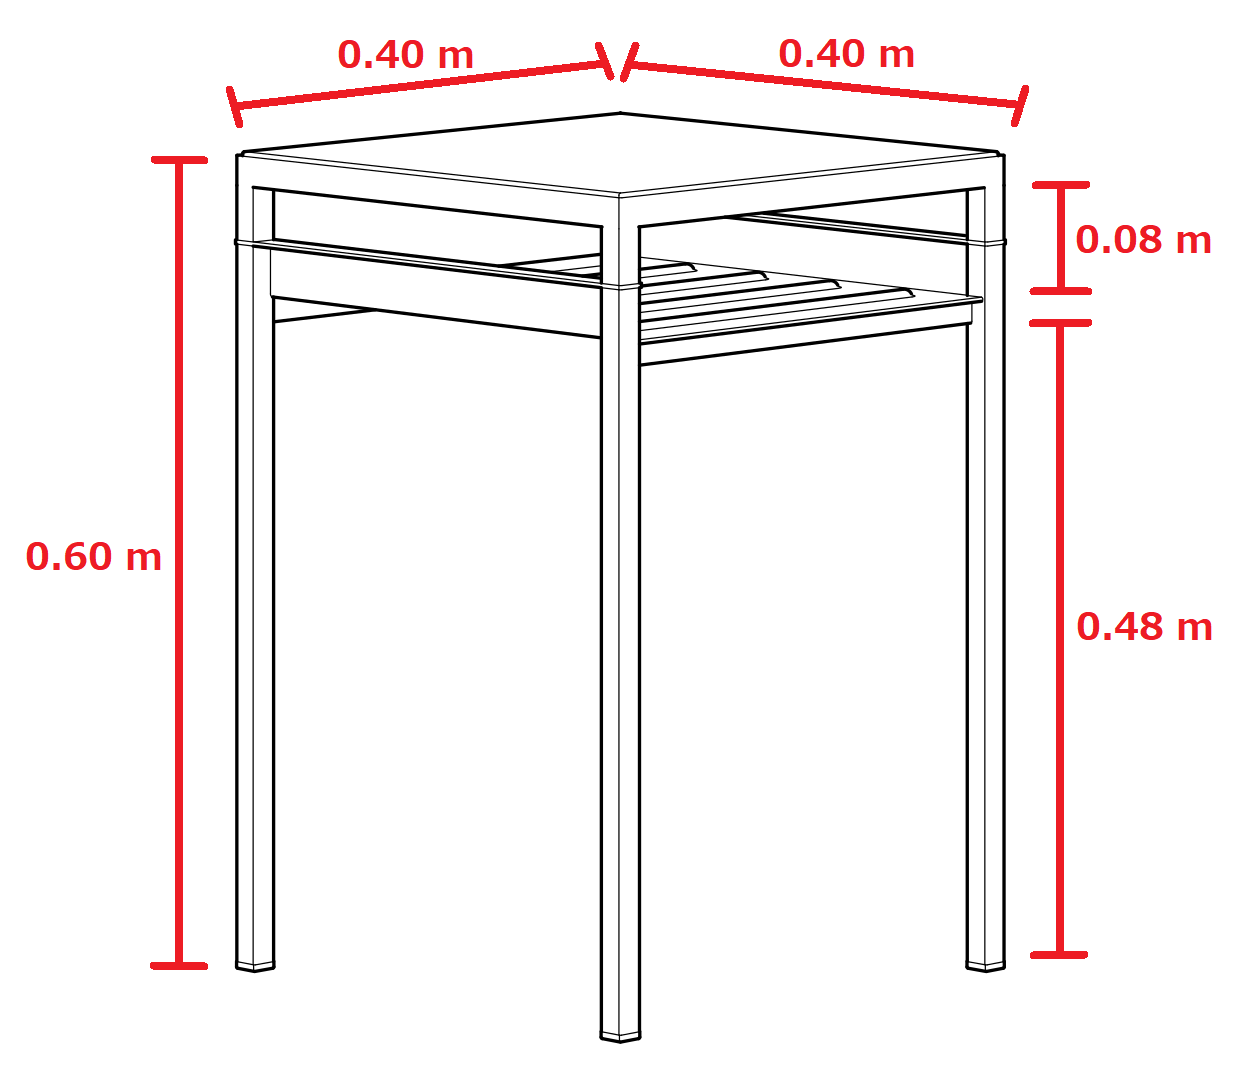
\includegraphics[width=0.80\textwidth]{{images/model_talltable.png}}
	\caption{Tall table model (width 0.40, length 0.40, height 0.60).}
	\label{fig:talltablemodel}
\end{figure}

\begin{figure}[!h]
	\centering
  	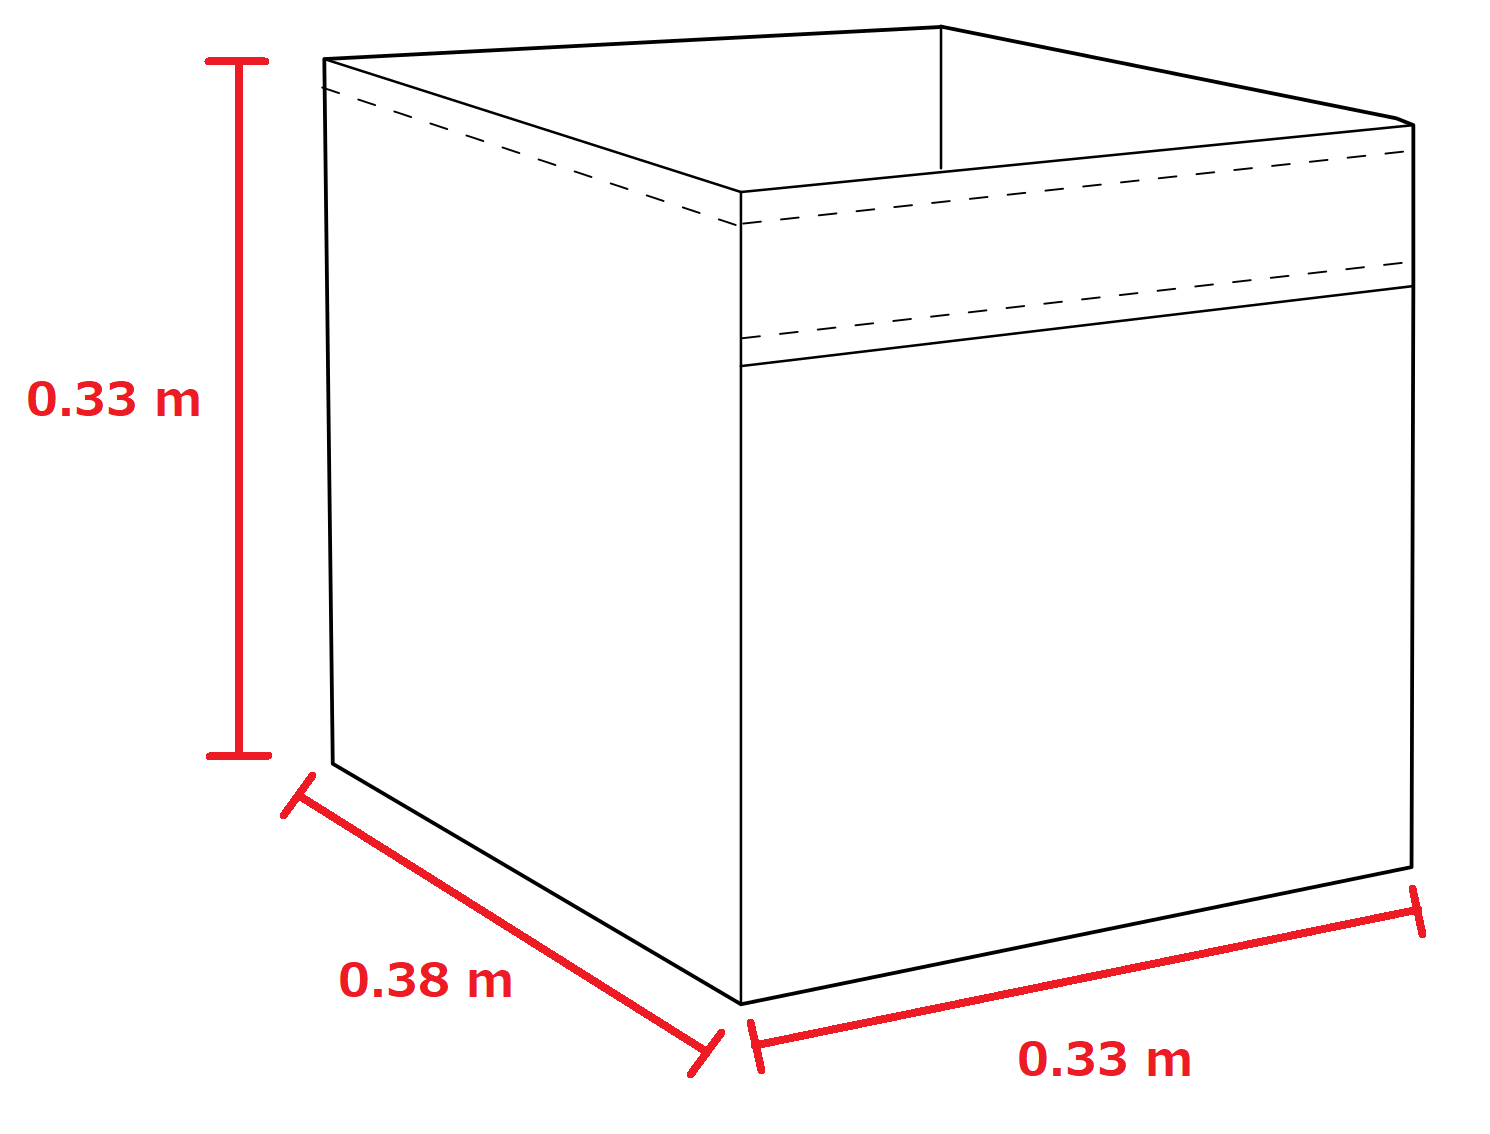
\includegraphics[width=0.80\textwidth]{{images/model_bin.png}}
	\caption{Bin model (width 0.38, length 0.33, height 0.33).}
	\label{fig:binmodel}
\end{figure}

\begin{figure}[!h]
	\centering
  	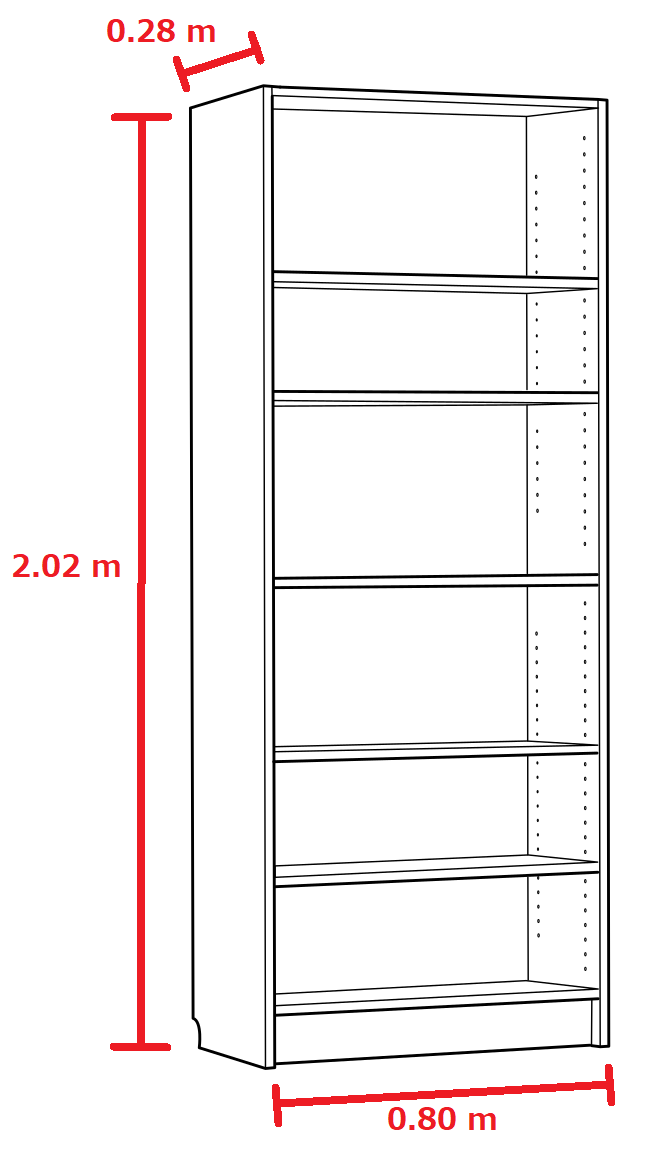
\includegraphics[width=0.80\textwidth]{{images/model_shelf.png}}
	\caption{Shelf model (width 0.28, length 0.80, height 2.02).}
	\label{fig:shelfmodel}
\end{figure}

\begin{figure}[!h]
	\centering
  	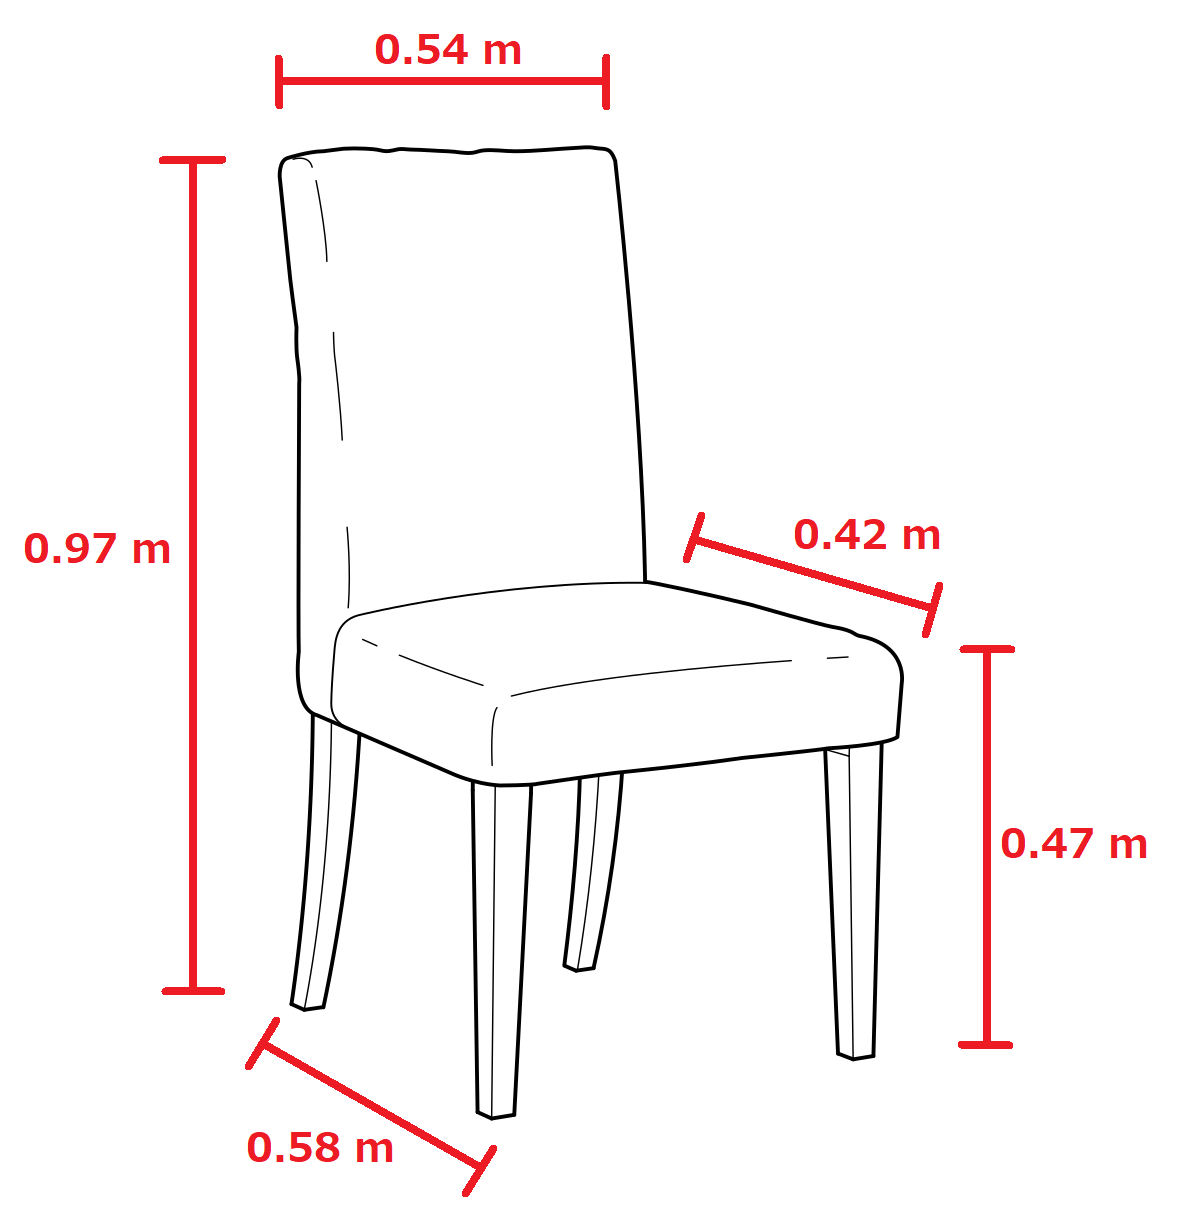
\includegraphics[width=0.80\textwidth]{{images/model_chair.png}}
	\caption{Chair model (width 0.58, length 0.54, height 0.97).}
	\label{fig:chairmodel}
\end{figure}

\clearpage
\subsection{Arena Setup}

The arena setup consists of two rooms (Room\_1 and Room\_2), one per task, as in Figure \ref{fig:arenaareas}. 

\subsubsection{Room 1}

In the Clean Up task, the room is divided in two main areas, the \textbf{Search Area}, where the objects are scattered around, and the \textbf{Deposit Area}, where the objects should be placed.

\begin{figure}[!h]%[!htbp]
	\centering
	%\begin{center}
	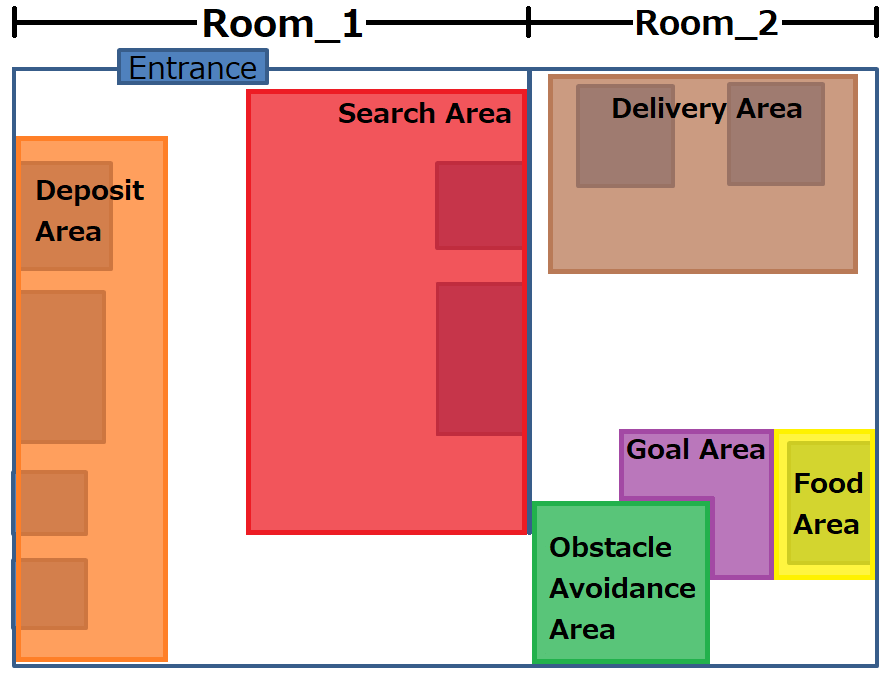
\includegraphics[width=0.80\textwidth]{{images/map_areas.png}}
	\caption{Test arena by interaction areas. There are two rooms, one per task, and five main areas: for Clean Up, in Room\_1, we have the Deposit and Search areas; in the case of Go and Get It, (Room\_2), for Task 2a we have the Obstacle Avoidance and Goal areas and, for Task 2b, the Food and Delivery areas.}
	\label{fig:arenaareas}
	%\end{center}
\end{figure}

The furniture regarding the Deposit Area includes the Drawer, Long Table, Bin\_A, and Bin\_B. In detail, the Drawer is divided in Drawer\_left, Drawer\_top, and Drawer\_bottom (see Figure \ref{fig:drawerstags}).

\begin{figure}[!h]%[!htbp]
	\centering
	%\begin{center}
	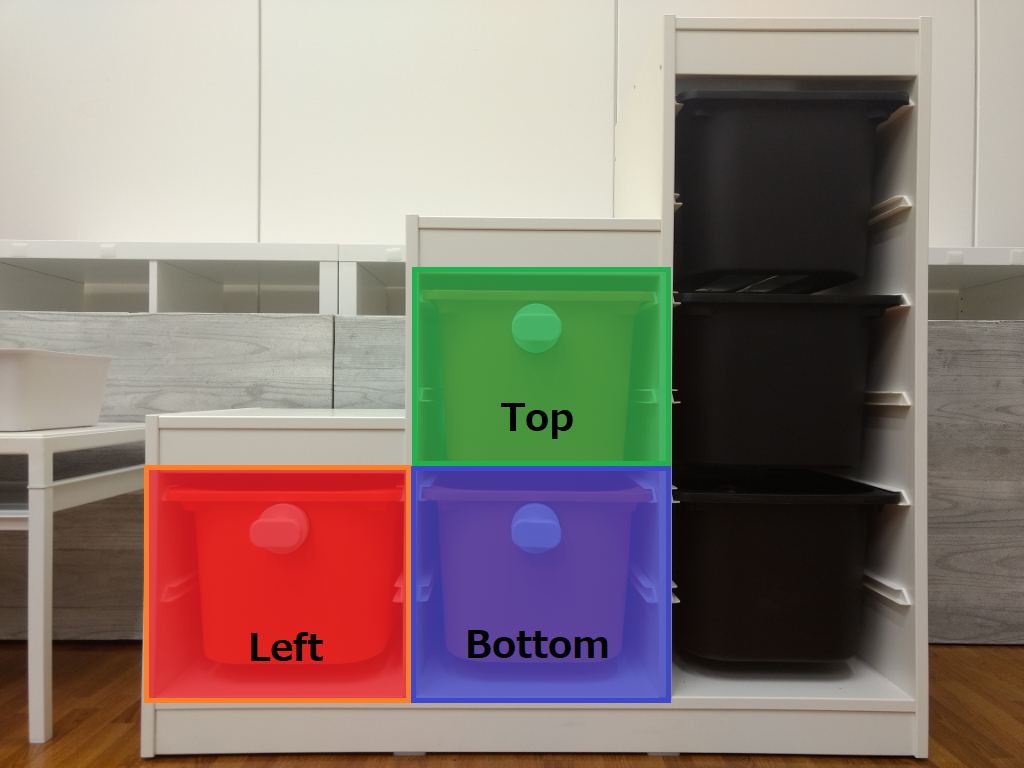
\includegraphics[width=0.80\textwidth]{{images/drawers_tags.png}}
	\caption{In the stairs-like drawer, only three drawers are going to be used, namely the Drawer\_left, and middle Drawer\_top and Drawer\_bottom.}
	\label{fig:drawerstags}
	%\end{center}
\end{figure}

Furthermore, the Long Table includes two types of deposits: tray and container. There are two similar trays (Tray\_A and Tray\_B) and two containers (Container\_A and Container\_B). The Container\_B should be small enough to contain markers/cutlery vertically in order to be able to evaluate the correct orientation and therefore we use the IKEA's Gessan container, as in \url{https://www.ikea.com/us/en/p/gessan-box-white-10371825/}.

\begin{figure}[!h]%[!htbp]
	\centering
	%\begin{center}
	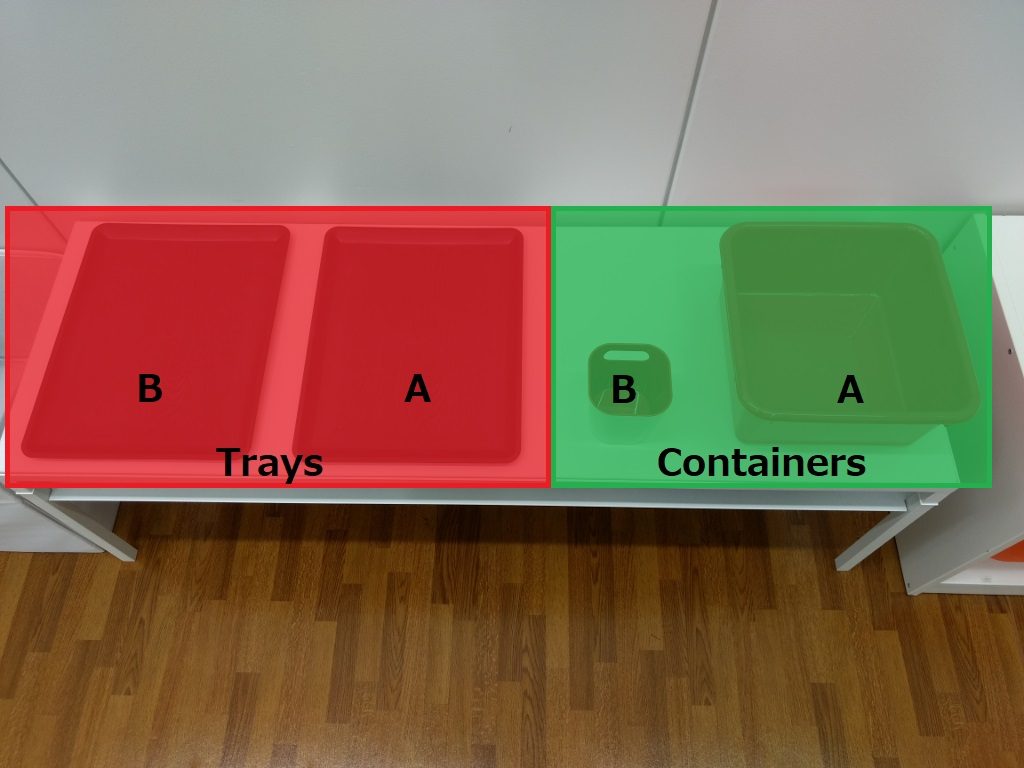
\includegraphics[width=0.80\textwidth]{{images/tray_container_tags.jpg}}
	\caption{In the Deposit Area, on the Long Table A there will be four deposits: Tray A, Tray B, Container A, and Container B. As a reference, the tray's size is 0.38 x 0.36 m, Container A is 0.28 x 0.28 x 0.125 m, and Container B is 0.095 x 0.095 m and 0.105 m height. Single color deposits are considered to detect any tag or mark that might be used as a reference.}
	\label{fig:containertags}
	%\end{center}
\end{figure}

A summary of the deposits per category can be found in Table \ref{table:deposits}. As a remainder, the object categories are as follows: Food (e.g. chips can, coffee can, cracker box), kitchen items (e.g. glass, bowl, mug), tools (e.g. screwdrivers, clamps, padlock and keys), shape items (e.g. baseball, tennis ball, foam brick), task items (e.g. Rubick’s cube, t-shirt, airplane toy), orientation-based items (e.g. markers, cutlery), and unknown objects.

\begin{table}[h!]
\begin{center}
\begin{tabular}{ |m{2.5cm}|m{2.5cm}|m{4.0cm}| } 
    \hline
    \begin{center} \textbf{Deposit} \end{center} & 
    \begin{center} \textbf{Place} \end{center} &
    \begin{center} \textbf{Category} \end{center}\\
    \hline
    Drawer\_left & Drawer & Shape items \\
    \hline
    Drawer\_top & Drawer & Tools \\
    \hline
    Drawer\_bottom & Drawer & Tools \\
    \hline
    Tray\_A & Long\_Table\_A & Food \\
    \hline
    Tray\_B & Long\_Table\_A & Food \\
    \hline
    Container\_A & Long\_Table\_A & Kitchen items \\
    \hline
    Container\_B & Long\_Table\_A & Orientation-based items \\
    \hline
    Bin\_A & Bin\_A & Task items\\
    \hline
    Bin\_B & Bin\_B & Unknown objects \\
    \hline
\end{tabular}
\end{center}
\caption{Object categories and their corresponding deposits in the arena, as in Figure \ref{fig:arena}.}
\label{table:deposits}
\end{table}

\subsubsection{Room 2}

Regarding Task 2a, the obstacles will be scattered around the access between rooms (i.e. the Obstacle Avoidance Area in Figure \ref{fig:arenaareas}), and they consist in flat and small objects bellow the laser height (as shown in Figure \ref{fig:obstacles}), therefore, other detection strategies should be implemented to be able to avoid them. The robot should navigate through the Obstacle Avoidance Area to a pre-announced goal location in the Goal Area.

\begin{figure}[!h]%[!htbp]
	\centering
	%\begin{center}
	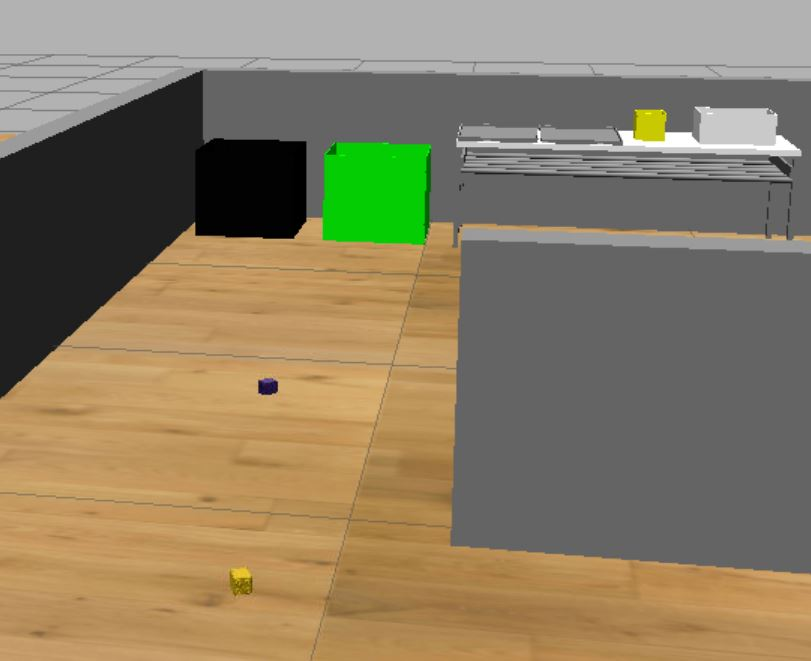
\includegraphics[width=0.80\textwidth]{{images/obstacles.jpg}}
	\caption{Obstacles laying on the rooms' access. They consist in small and or flat objects.}
	\label{fig:obstacles}
	%\end{center}
\end{figure}

In Task 2b, the food items in the Food Area will be placed inside a shelf (Figure \ref{fig:shelf} and Figure \ref{fig:shelfmodel}) with board levels at 0.50 m, 0.80 m, and 1.05 m height and three different depths: front, middle, and back, as shown in Figure \ref{fig:shelfobjects}. The target object may be at any depth and therefore a grasping strategy should be developed to softly move the objects obstructing the requested drink as necessary (e.g. if the requested item is in the middle level and middle depth, first move any object in the front depth to a different level before being able to grasp the requested food).

\begin{figure}[!h]%[!htbp]
	\centering
	\begin{subfigure}{.45\textwidth}
  		\centering
	    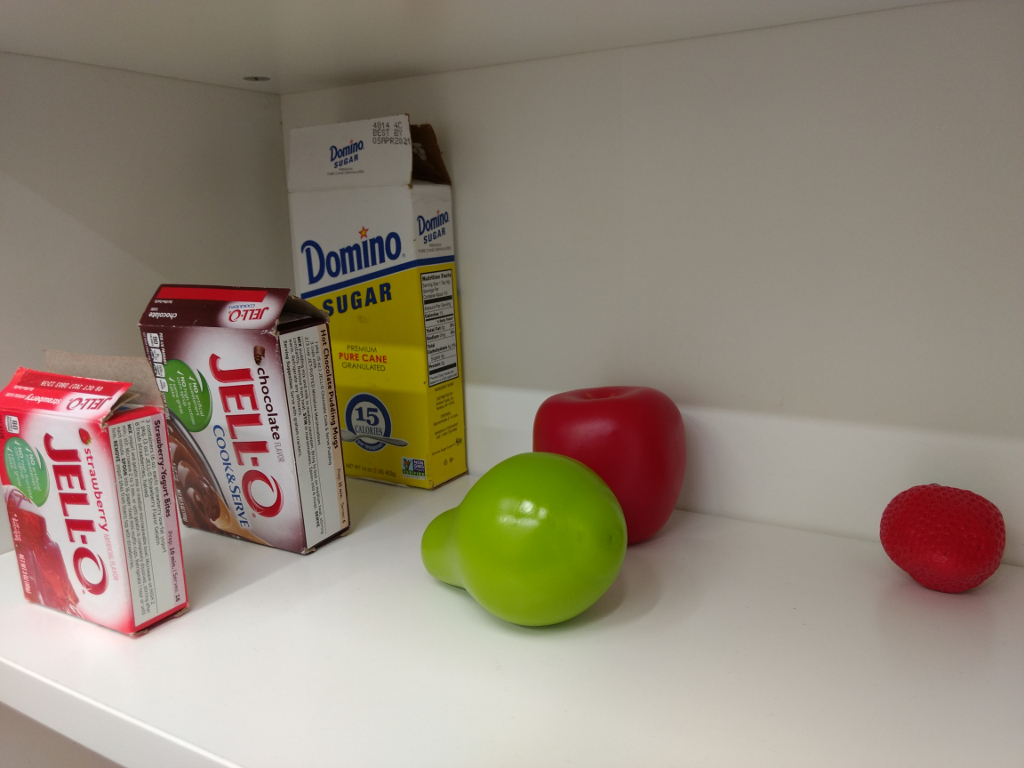
\includegraphics[width=1\textwidth]{{images/shelf_objects_a.jpg}}
	    \caption{}
  		\label{fig:shelfobjectsa}
	\end{subfigure}
	\begin{subfigure}{.45\textwidth}
  		\centering
  		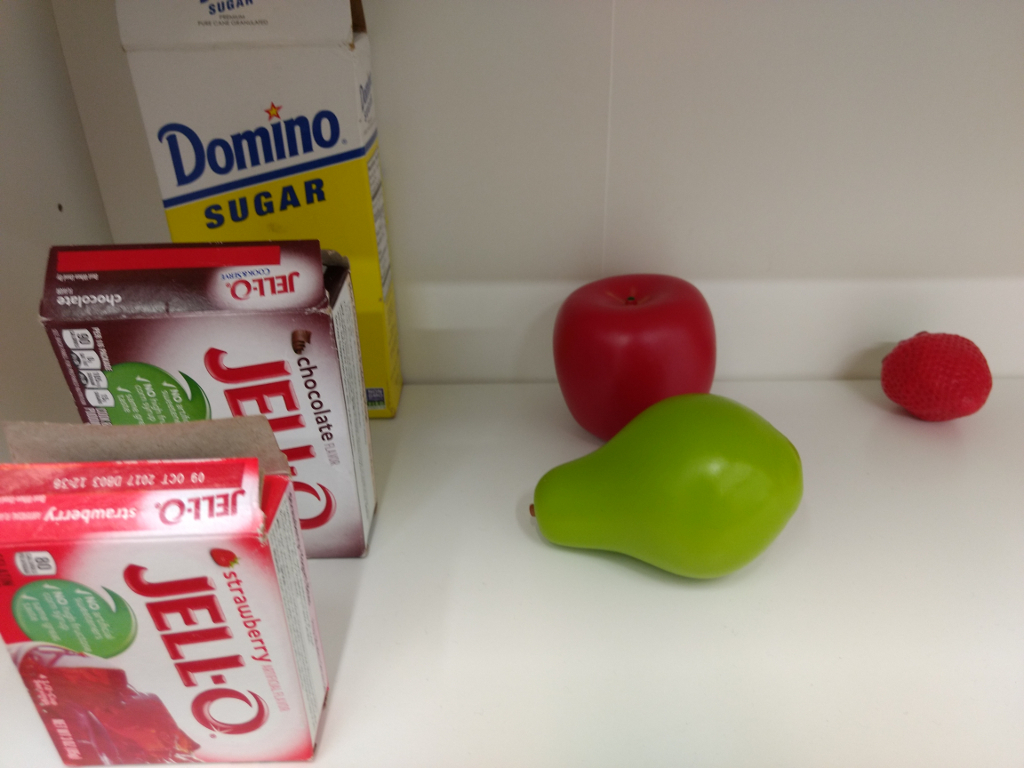
\includegraphics[width=1\textwidth]{{images/shelf_objects_b.jpg}}
  		\caption{}
  		\label{fig:shelfobjectsb}
	\end{subfigure}
	\caption{a) Lateral and b) front views of the objects' distribution at three different depths (front, middle and back).}
	\label{fig:shelfobjects}
	%\end{center}
\end{figure}

Finally, there will be two persons in the Delivery Area (they might be either standing up or sitting down) and one of them will be requesting an item by waving her/his arm (it can be both the left or right arm).

\clearpage
\subsection{Objects to be used}

Object's specifications and their corresponding 3D models can be found in \url{http://www.ycbbenchmarks.com} . Mass and weight can be consulted in \url{http://www.ycbbenchmarks.com/wp-content/uploads/2015/09/object-list-Sheet1.pdf}.

IMPORTANT: \textbf{Object availability}: Please consider that some objects might be no longer available and might be replaced by an equivalent object based on availability and similarly in dimensions and visual appearance. For details and updates, please check the following site: \url{https://www.uml.edu/Research/NERVE/YCB-Form.aspx} . We will let you know in advance the dataset to be used during the competition.

\begin{itemize}
    \item Food items:
        \SubItem{Cheez-it cracker box}
        \SubItem{Domino sugar box}
        \SubItem{Jell-o chocolate pudding box}
        \SubItem{Jell-o strawberry gelatin box}
        \SubItem{Spam potted meat can}
        \SubItem{Master chef coffee can}
        \SubItem{Starkist tuna fish can}
        \SubItem{Pringles chips can}
        \SubItem{French's mustard bottle}
        \SubItem{Tomato soup can}
        \SubItem{Plastic banana}
        \SubItem{Plastic strawberry}
        \SubItem{Plastic apple}
        \SubItem{Plastic lemon}
        \SubItem{Plastic peach}
        \SubItem{Plastic pear}
        \SubItem{Plastic orange}
        \SubItem{Plastic plum}
    \item Kitchen items:
        \SubItem{Windex Spray bottle}
        \SubItem{Srub cleanser bottle}
        \SubItem{Scotch brite dobie sponge}
        \SubItem{Pitcher base}
        \SubItem{Pitcher lid}
        \SubItem{Plate}
        \SubItem{Bowl}
        \SubItem{Fork}
        \SubItem{Spoon}
        \SubItem{Spatula}
        \SubItem{Wine glass}
        \SubItem{Mug}
    \item Tool items:
        \SubItem{Large marker}
        \SubItem{Small marker}
        \SubItem{Keys (from the Padlock)}
        \SubItem{Bolt and nut}
        \SubItem{Clamps}
    \item Shape items:
        \SubItem{Credit card blank}
        \SubItem{Mini soccer ball}
        \SubItem{Soft ball}
        \SubItem{Baseball}
        \SubItem{Tennis ball}
        \SubItem{Racquetball}
        \SubItem{Golf ball}
        \SubItem{Marbles}
        \SubItem{Cups}
        \SubItem{Foam brick}
        \SubItem{Dice}
        \SubItem{Rope}
        \SubItem{Chain}
    \item Task items:
        \SubItem{Rubik's cube}
        \SubItem{Colored wood blocks}
        \SubItem{9-peg-hole test}
        \SubItem{Toy airplane}
        \SubItem{Lego duplo}
        \SubItem{Magazine}
        \SubItem{Black t-shirt}
        \SubItem{Timer}

    %\item Hard-to-manipulate:

    \item Discarded:
        \SubItem{Skillet}
        \SubItem{Skillet lid}
        \SubItem{Table cloth}
        \SubItem{Hammer}
        \SubItem{Adjustable wrench}
        \SubItem{Wood block}
        \SubItem{Power drill}
        \SubItem{Washers}
        \SubItem{Nails}
        \SubItem{Knife}
        \SubItem{Scissors}
        \SubItem{Padlock}
        \SubItem{Phillips screwdriver}
        \SubItem{Flat screwdriver}
        \SubItem{Clear box}
        \SubItem{Box lid}
        \SubItem{Footlocker}
\end{itemize}

\end{document}

